\documentclass{tum_report}

\bibliographystyle{tex_files/bibliography/styles/iso690}

% Make \paragraph a block heading (new line after it)
\usepackage{titlesec}
\titleformat{\paragraph}[block]
  {\normalfont\normalsize\bfseries}
  {\theparagraph}{1em}{}
\titlespacing*{\paragraph}{0pt}{1.2ex}{0.6ex}

\usepackage{float}
\usepackage{placeins}
\usepackage{forest}
\usepackage{adjustbox}
\usepackage{pdfpages}
\usepackage{appendix}

\forestset{
  daqtree/.style={
    for tree={
      draw,
      rounded corners,
      align=center,
      parent anchor=south,
      child anchor=north,
      edge={->},
      l sep=10pt,
      s sep=6pt,
      font=\ttfamily\small
    }
  }
}

\newcommand{\bnf}[1]{\texttt{\langle #1 \rangle}}

\begin{document}

    \ministry{Ministry of Education, Culture and Research of Republic of Moldova}
\university{Technical University of Moldova}
\faculty{Faculty of Computers, Informatics and Microelectronics}
\department{Department of Software Engineering and Automatics}

\title{DaQuVa: Data Quality Validator.}{Some DSL blabla bla.}

\year{2026}


\begin{titlepage}

    \textsc{\ministryname} \\
    \textsc{\universityname} \\
    \textsc{\facultyname} \\
    \textsc{\departmentname} \\
	
	\vfill
	
	{\LARGE \titleen \par}
	{\LARGE DSL  \par}
	
	\vfill
    	
    \begin{table}[h!]
        \hfill
        \begin{tabular}{lr}
        \textbf{Mentor:}   & \supervisor{prof.}{Vladislav Crucerescu} \\
        \textbf{Students:} & \student{Cimendur Rustem}{FAF-243}  \\
                           & \student{Frunza Damian}{FAF-243}       \\
                           & \student{Pancenco Mihail}{FAF-243}    \\
                           & \student{Tureac Daria}{FAF-243}\end{tabular}
    \end{table}
	
	\vfill

	{Chișinău, \degreeyear \par}

\end{titlepage}
    \clearpage

    \chapter*{Abstract}

Modern relational databases increasingly suffer from data quality problems
including inconsistencies, duplicates, missing values, and constraint violations
arising from heterogeneous data sources and evolving business rules. Existing
solutions, ranging from interactive visual tools and SQL-based rule engines to
enterprise data quality platforms and DSL-based pipeline frameworks, either embed
validation logic in graphical interfaces or proprietary configurations, or focus
on data transformation pipelines rather than on an explicit, reusable, and
auditable specification of data quality constraints. This paper presents DaQuVa
(Data Quality Validator), a novel domain-specific language designed to address
these gaps by providing a declarative, safety-first approach to data quality
enforcement in SQL databases. DaQuVa introduces a formally defined grammar, a
sequential execution model, and a constrained expression language that makes
programs straightforward to review and audit. The language provides core
constructs for column-level scanning via pluggable validation tools,
threshold-based filtering, local duplicate detection with optional AI-powered
similarity scoring, controlled database writes through an explicit safety
mechanism (\texttt{allowDanger}), result export to multiple sinks, and modular
reusability through parameterized functions. A Python-based implementation
comprising a regex-driven lexer, a recursive-descent parser, and an execution
engine is described. Experimental evaluation demonstrates that DaQuVa can detect
and flag erroneous records and near-duplicate entries across realistic datasets
with concise, human-readable scripts, while its safety constraints prevent
accidental data loss. Unlike general-purpose DSLs or tool-driven approaches,
DaQuVa treats data quality rules as a formal, portable contract between technical
teams and domain experts, contributing a practical foundation for reproducible
and auditable data quality management.
 
    \clearpage

    \addtocontents{toc}{\protect \thispagestyle{empty}}
    \tableofcontents
    \thispagestyle{empty}
    \clearpage

    \addcontentsline{toc}{chapter}{Introduction}
\chapter*{Introduction}

%this intro is a bullshit. Need to come back after all other report will be done. For now I leave it here as a temp-for-them-tipa Zatichka

\par Data cleaning is a fundamental process aimed at detecting and correcting errors, inconsistencies, and redundancies in data to ensure high data quality, especially in large-scale systems such as data warehouses, federated databases, and web-based information platforms. Due to the heterogeneity, volume, and continuous evolution of modern data sources, effective data cleaning requires systematic, scalable, and declarative approaches that minimize manual effort while ensuring correctness and reproducibility \cite{rahm2000data}.

Consequently, there is a growing demand for expressive, scalable, and systematic frameworks that enable users to specify, detect, and repair data quality issues in a declarative and reusable manner. This motivates the development of domain-specific abstractions and languages that can bridge the gap between conceptual data quality requirements and their practical implementation in modern data processing pipelines \cite{chu2016datacleaning,rahm2000data}.

Interactive data cleaning systems, such as Potter's Wheel, address the limitations of traditional batch-oriented approaches by tightly integrating discrepancy detection with data transformations. This allows users to iteratively refine cleaning operations on large and heterogeneous datasets through immediate feedback, graphical specifications, and automatic inference of domain structures, reducing the need for complex programming and repeated manual inspection \cite{raman2001potterswheel}.

Wrangler is an interactive system for data transformation that combines direct manipulation of visualized data with automatic inference of applicable transforms. It enables analysts to iteratively clean, reshape, and validate data while capturing an auditable script of all transformations, reducing manual effort and improving reusability \cite{kandel2011wrangler}.

    \clearpage

    \chapter{Domain Analysis}
% Rustam's work goes here:


\section{Problem statement}
\section{Motivation and need for DSL}

% Despite they are our concurents, the imperical reserch says that DSL in general helped, so, it is usefull to implement it. We use this info. 
% https://www.arxiv.org/pdf/2505.16764
%

% may be here about that it is needed for AI
% https://dl.acm.org/doi/epdf/10.1145/3329486.3329493


% use also introduction from other articles where all them says that data cleaning takes more than 50% of data guys

\section{Target Audience}
% From some of these papers also take this already written section about target audience. It already has been written

\section{Existing solutions analysis}
%should be tables for comparative analysis

\subsection{Non-DSL solutions}

Non-DSL solutions represent the historically dominant way of addressing data quality and data cleaning tasks. Instead of offering a dedicated declarative language, these approaches rely on interactive graphical interfaces, visual specification techniques, enterprise platforms, or direct SQL expressions. As a result, they effectively tackle many practical cleaning scenarios, but they tend to encode quality logic in tools, workflows, or queries rather than in an explicit, reusable language of data quality rules.

\paragraph{Visual modeling and UML-based quality approaches.}
One direction is to use visual modeling notations such as UML to describe data structures, constraints, and quality requirements on a conceptual level \cite{quality-assessment-uml}. 
Such approaches help stakeholders reason about completeness, consistency, and other quality attributes of models, but they do not directly execute validation rules on concrete SQL tables and typically require an additional implementation step in code or database constraints. 

\begin{table}[h]
\centering
\caption{Visual UML-based approaches: pros and cons}
\begin{tabular}{|p{0.45\linewidth}| p{0.45\linewidth}|}
\hline
\textbf{Advantages} & \textbf{Limitations} \\
\hline
Expressive visual notation for structures and constraints, accessible to architects and analysts. &
Models are descriptive only; quality rules are not directly executable on concrete datasets. \\
Facilitates discussion of data quality attributes (completeness, consistency) at design time. &
Requires a separate implementation step in SQL, application code, or ETL tools, which can diverge from the model. \\
Supports continuous quality assessment and improvement of models themselves. &
Focuses on model-level quality rather than operational validation of large SQL tables in production. \\
\hline
\end{tabular}
\end{table}

\paragraph{Interactive visual data transformation tools (Wrangler).}
Wrangler is an interactive system for specifying data transformation scripts through direct manipulation of tabular data \cite{wrangler}. 
Analysts iteratively select parts of the dataset, and Wrangler suggests applicable transformations, previews their effects, and records an auditable transformation history \cite{wrangler}. 
Although Wrangler internally relies on a declarative transformation language, users mainly see a visual interface for shaping and cleaning data, rather than an explicit, reusable language of quality rules.

\begin{table}[h]
\centering
\caption{Wrangler: pros and cons}
\begin{tabular}{|p{0.45\linewidth}| p{0.45\linewidth}|}
\hline
\textbf{Advantages} & \textbf{Limitations} \\
\hline
Interactive visual interface for specifying complex data transformations without manual scripting. &
Focuses on one-off or pipeline-oriented transformations, not on explicit reusable data quality constraints. \\
Mixed-initiative suggestions help users quickly discover useful cleaning operations. &
Underlying transformation language is hidden; rules are not exposed as a stable, human-readable contract. \\
Maintains an auditable history of transformations that can be replayed. &
Primarily designed for pre-analytics data wrangling rather than continuous validation of SQL tables in production. \\
\hline
\end{tabular}
\end{table}

\paragraph{Interactive and deterministic data repair (Falcon).}
Falcon is an interactive data cleaning system that uses SQL \texttt{UPDATE} queries as the underlying repair language and focuses on deterministic, explainable modifications \cite{falcon}. 
It encourages users to iteratively explore the space of candidate repairs, presents them as concrete SQL updates, and evaluates their impact on the data \cite{falcon}. 
However, Falcon assumes that users are comfortable reasoning about SQL repairs and does not provide a separate, higher-level vocabulary for stating business-level data quality requirements. 

\begin{table}[h]
\centering
\caption{Falcon: pros and cons}
\begin{tabular}{|p{0.45\linewidth}| p{0.45\linewidth}|}
\hline
\textbf{Advantages} & \textbf{Limitations} \\
\hline
Produces deterministic, explainable repairs in the form of explicit SQL \texttt{UPDATE} statements. &
Assumes users can understand and validate SQL-level repair queries, which may be too low-level for domain experts. \\
Supports interactive exploration of alternative repairs and their impact on the dataset. &
Does not define a separate declarative language of data quality rules; repairs are not tied to an explicit rule set. \\
Integrates naturally with relational databases by operating directly on SQL tables. &
Focuses on fixing specific instances of dirty data rather than establishing a reusable, auditable quality contract for future data. \\
\hline
\end{tabular}
\end{table}

\paragraph{General-purpose interactive cleaning tools (OpenRefine).}
OpenRefine is a widely used open-source tool for cleaning and transforming tabular data via a spreadsheet-like interface \cite{openrefine-site}. 
It supports faceted browsing, clustering similar values, reconciliation with external data sources, and an undo/redoable history of operations that can be replayed on new datasets \cite{openrefine-site}. 
OpenRefine is highly effective for one-off or exploratory data cleaning tasks, but its operations are not designed to serve as a formal and reusable contract of data quality for production SQL databases. 

\begin{table}[h]
\centering
\caption{OpenRefine: pros and cons}
\begin{tabular}{|p{0.45\linewidth}| p{0.45\linewidth}|}
\hline
\textbf{Advantages} & \textbf{Limitations} \\
\hline
User-friendly, spreadsheet-like interface suitable for analysts working with messy CSV or JSON data. &
Primarily a desktop/GUI tool; not natively integrated as an automated, repeatable check within database pipelines. \\
Powerful features for clustering similar values, faceted filtering, and reconciliation with external sources. &
Cleaning operations are sequences of GUI actions or expressions, not explicit, reusable data quality rules over SQL tables. \\
Supports undo/redo and operation history that can be applied to similar datasets. &
Better suited for ad-hoc or exploratory cleaning than for serving as a formal data quality contract in production environments. \\
\hline
\end{tabular}
\end{table}

\paragraph{Enterprise data quality platforms.}
Large vendors such as IBM, Oracle, or SAS provide comprehensive data quality platforms that combine profiling, cleansing, standardisation, and matching capabilities \cite{rahm2000data}. 
These tools typically integrate tightly with existing ETL and MDM solutions, offer rich dashboards, and support complex matching and deduplication rules for customer or product data. 
They address enterprise-wide governance requirements but come with significant cost and operational complexity.

\begin{table}[h]
\centering
\caption{Enterprise data quality platforms: pros and cons}
\begin{tabular}{|p{0.45\linewidth}| p{0.45\linewidth}|}
\hline
\textbf{Advantages} & \textbf{Limitations} \\
\hline
Comprehensive feature set, including profiling, cleansing, matching, and enrichment across many data sources. &
High licence and infrastructure costs, typically only justified for large organisations. \\
Tight integration with existing ETL, MDM, and governance tools, enabling end-to-end management of data quality. &
Configuration is often complex; setting up rules and workflows requires specialised consultants or trained staff. \\
Rich dashboards and monitoring for continuous tracking of quality metrics at scale. &
Business rules are embedded as configuration artefacts inside the platform, not as a lightweight, portable language over SQL tables. \\
\hline
\end{tabular}
\end{table}

\paragraph{SQL-based rule engines and database-centric checks.}
Another class of solutions relies directly on SQL expressions and stored procedures to implement data quality checks and remediation logic \cite{rahm2000data}. 
Teams define validation rules as SQL queries or views that flag invalid rows, and sometimes tie them to scheduling and alerting via ETL or orchestration tools. 
This approach keeps rules close to the database but can become fragmented and hard to audit as the number of checks grows.

\begin{table}[h]
\centering
\caption{SQL-based rule engines: pros and cons}
\begin{tabular}{|p{0.45\linewidth}| p{0.45\linewidth}|}
\hline
\textbf{Advantages} & \textbf{Limitations} \\
\hline
Uses standard SQL, which is widely known among data engineers and easy to execute in existing databases. &
Rules are scattered across queries, views, and stored procedures, making them hard to discover and maintain. \\
Allows fine-grained control and optimisation of checks for specific schemas and performance constraints. &
SQL syntax is verbose for complex business rules and not easily readable by non-technical stakeholders. \\
Can be integrated into existing ETL pipelines and CI/CD workflows without introducing new runtime components. &
Rules are not expressed as a single, declarative contract; there is no unified catalogue of quality expectations per table. \\
\hline
\end{tabular}
\end{table}

\paragraph{Data profiling and catalog tools with quality rules.}
Data catalog and profiling tools provide automated statistics, distributions, and anomaly detection over database tables and columns. 
Some of them allow users to attach simple quality rules (for example, thresholds on null rates or uniqueness) and to track violations over time in a central dashboard. 
They are effective for discovering issues and monitoring trends but typically offer only a limited rule language focused on basic metrics.

\begin{table}[h]
\centering
\caption{Profiling and catalog tools: pros and cons}
\begin{tabular}{|p{0.45\linewidth}| p{0.45\linewidth}|}
\hline
\textbf{Advantages} & \textbf{Limitations} \\
\hline
Automatically compute descriptive statistics and distributions that reveal hidden data quality problems. &
Rule definition is usually restricted to simple thresholds on precomputed metrics (null rate, distinct count, etc.). \\
Centralises quality metrics and rule evaluations in dashboards that are accessible to many stakeholders. &
Do not provide an expressive, table-focused language for complex, cross-column business constraints. \\
Help prioritise where to invest cleaning effort by highlighting high-risk tables and columns. &
Monitoring is often decoupled from actual repair workflows; suggestions for fixes are weak or absent. \\
\hline
\end{tabular}
\end{table}

\paragraph{Self-service analytics tools with built-in validation.}
Self-service analytics platforms often include basic validation and cleansing functions within their visual workflows. 
Business users can define filters, simple constraints, and data type checks directly in a drag-and-drop interface and reuse these flows across reports. 
This reduces the need for ad-hoc scripting but keeps validation logic tied to specific reports rather than to the underlying database tables.

\begin{table}[H]
\centering
\caption{Self-service analytics tools: pros and cons}
\begin{tabular}{|p{0.45\linewidth}| p{0.45\linewidth}|}
\hline
\textbf{Advantages} & \textbf{Limitations} \\
\hline
Accessible to non-technical users through visual workflows and predefined cleaning components. &
Validation rules are often bound to particular reports or dashboards, not to shared database schemas. \\
Enable rapid creation of reusable cleaning and transformation steps inside analytical pipelines. &
Rule logic remains hidden inside proprietary workflow definitions, hindering auditing and cross-team reuse. \\
Reduce dependency on engineering teams for basic validation and filtering tasks. &
Not designed as a general-purpose data quality layer with an explicit, portable specification of rules. \\
\hline
\end{tabular}
\end{table}

\FloatBarrier
\paragraph{Summary}
Overall, non-DSL solutions demonstrate that interactive visual tools, SQL-based repair systems, enterprise platforms, and profiling tools can substantially reduce manual data cleaning effort and improve transparency of transformations \cite{rahm2000data,wrangler,openrefine-site}. 
At the same time, they either lack a dedicated, human-readable language for expressing reusable data quality rules over SQL tables, or they hide such a language behind configuration and GUIs, which makes it difficult to treat these rules as an explicit, auditable contract between technical and business stakeholders \cite{falcon,quality-assessment-uml}.








\subsection{Existing DSL solutions}
% Misa's work goes here:

% direct competent
In contrast to non-DSL approaches, a number of research works and industrial systems propose the use of domain-specific languages (DSLs) for data cleaning, transformation, and data quality management. 
The core idea behind these approaches is to provide a formal, high-level, and declarative way of specifying data processing logic and quality constraints, closely aligned with domain semantics rather than low-level implementation details.

DSL-based solutions typically aim to improve readability, maintainability, and reusability of data cleaning workflows, while enabling explicit and machine-executable specifications of business rules. 
Empirical studies indicate that the use of DSLs can significantly increase productivity and reduce error rates in complex data manipulation tasks \cite{dsl-empirical-2025}. 
As a result, DSLs are increasingly explored as a systematic alternative to ad-hoc scripting and purely tool-driven approaches.

One representative example of such a language is \textbf{Jayvee} \cite{jayvee}, a domain-specific language and execution framework for modeling data processing pipelines together with integrated data quality logic.

Conceptually, Jayvee treats data processing as a formally defined \emph{pipeline model}. 
A pipeline is a strictly ordered sequence of computational units called \emph{blocks}, where the output of each block becomes the input of the next one. 
This enforces an explicit, linear dataflow model that makes transformations, dependencies, and execution order unambiguous.

Jayvee defines three fundamental categories of blocks:
\begin{itemize}
    \item \textbf{Extractor blocks} — model data sources (e.g., HTTP endpoints, filesystems, databases) and introduce data into the pipeline.
    \item \textbf{Transformator blocks} — perform structured transformations, filtering, selection, and interpretation of intermediate data representations.
    \item \textbf{Loader blocks} — represent data sinks and persist processed data into storage systems.
\end{itemize}

This architecture maps directly to the classical ETL (Extract--Transform--Load) paradigm, but formalizes it as a typed, declarative pipeline language rather than as scripts or tool configurations.

A central design element of Jayvee is its \emph{type system based on value types}. 
Instead of treating data as untyped strings or generic table cells, Jayvee allows users to define domain-specific value types (e.g., percentages, identifiers, measurements) and attach \emph{formal constraints} to them. 
These constraints define admissible value ranges, formats, and semantic properties, and are evaluated automatically during pipeline execution. 
As a result, data quality validation becomes an intrinsic part of the execution semantics, not an external checking step.

Jayvee also supports \emph{explicit transformation definitions} that map values between types, enabling controlled and traceable semantic conversions (e.g., unit conversions, format normalization). 
Furthermore, it allows the definition of \emph{composite block types}, which are higher-level abstractions composed of multiple basic blocks. 
This enables modularization, reuse, and abstraction of complex processing logic into reusable components.

From a software engineering perspective, Jayvee can be classified as a \emph{typed dataflow DSL} that exhibits:
\begin{itemize}
    \item an explicit and structured pipeline model,
    \item formally specified computational units,
    \item a domain-oriented type system,
    \item built-in constraint-based data validation, and
    \item mechanisms for modular composition and reuse.
\end{itemize}
Consequently, Jayvee transcends traditional transformation scripting and serves as a formal modeling language for data pipelines with integrated data quality semantics.


\begin{table}[h]
\centering
\caption{Jayvee: advantages and limitations}
\begin{tabular}{|p{0.45\linewidth}| p{0.45\linewidth}|}
\hline
\textbf{Advantages} & \textbf{Limitations} \\
\hline
Formal pipeline model with explicit dataflow semantics and execution order. &
Requires learning a new language and modeling paradigm compared to SQL-based solutions. \\
\hline
Strong domain-oriented type system with value types and constraints. &
Less flexible for highly dynamic or unstructured data compared to script-based approaches. \\
\hline
Integrated data quality validation as part of execution semantics. &
Primarily focused on structured pipelines; not designed for ad-hoc exploratory cleaning. \\
\hline
Clear separation of extraction, transformation, and loading stages. &
Depends on predefined block types for integration with external systems. \\
\hline
Support for modular composition via composite blocks and reusable components. &
Smaller ecosystem compared to mature enterprise ETL platforms. \\
\hline
Declarative, readable specification of complex data workflows. &
Requires formal modeling effort even for simple pipelines. \\
\hline
\end{tabular}
\end{table}

% https://jvalue.github.io/jayvee/ 


% It sais that it is a library AND a DSL, so.. need to be here
% https://link.springer.com/chapter/10.1007/978-3-319-47602-5_27
\paragraph{Grafter and Grafterizer.}
Another representative DSL-based approach is \textbf{Grafter}, together with its interactive environment \textbf{Grafterizer} \cite{grafterizer}. 
Grafter is implemented as an embedded domain-specific language (eDSL) in the functional programming language Clojure, targeting data cleaning, transformation, and semantic data publishing workflows. 
While syntactically realized as a software library, Grafter introduces a dedicated abstraction layer for expressing domain-level data transformation pipelines, thereby fulfilling the defining characteristics of a DSL.

Conceptually, Grafter follows a \emph{functional pipeline model}, where data transformations are represented as composable functions, called \emph{pipes}. 
Each pipe performs a single, well-defined transformation step, and complex workflows are constructed through functional composition. 
This model enforces a clear and explicit dataflow structure, in which intermediate results are immutable and transformation semantics are deterministic, enabling transparent reasoning about pipeline behavior.

A distinctive feature of Grafter is its strong integration of \emph{data cleaning and semantic transformation}. 
In addition to conventional tabular cleaning operations such as filtering, normalization, enrichment, and value derivation, Grafter provides first-class constructs for mapping cleaned data into RDF representations. 
Users define semantic mappings using explicit triple generation rules, enabling the transformation of raw tabular data into Linked Data formats suitable for publication and semantic interoperability.

Grafterizer extends the Grafter DSL by providing an interactive graphical environment for constructing, testing, and executing transformation pipelines. 
Through a visual interface, users can compose pipelines from predefined transformation operators, preview intermediate results, and iteratively refine workflows. 
This interactive layer lowers the barrier of entry for domain experts while preserving the expressive power and compositional semantics of the underlying DSL.

From a software engineering perspective, Grafter can be classified as a \emph{functional embedded DSL} characterized by:
\begin{itemize}
    \item compositional transformation pipelines,
    \item functional abstraction and immutability,
    \item explicit dataflow modeling,
    \item extensible operator libraries, and
    \item integrated semantic data mapping.
\end{itemize}
This design makes Grafter particularly suitable for large-scale data transformation and semantic publishing workflows, while Grafterizer facilitates interactive development and validation of data cleaning logic.

\begin{table}[h]
\centering
\caption{Grafter and Grafterizer: advantages and limitations}
\begin{tabular}{|p{0.45\linewidth}| p{0.45\linewidth}|}
\hline
\textbf{Advantages} & \textbf{Limitations} \\
\hline
Functional pipeline DSL enables modular, compositional data transformations. &
Requires understanding of functional programming concepts, which may be unfamiliar to many data analysts. \\
\hline
Integrated support for both data cleaning and RDF generation within a single language framework. &
Strong orientation toward semantic web workflows limits applicability to purely relational or analytical pipelines. \\
\hline
Clear and explicit dataflow semantics improve reasoning about transformation correctness. &
Embedded DSL syntax inherits complexity from the host language (Clojure). \\
\hline
Interactive graphical interface supports incremental pipeline development and debugging. &
Graphical abstraction may obscure underlying transformation semantics for advanced users. \\
\hline
Extensible through custom transformation operators and semantic mappings. &
Custom extensions require proficiency in Clojure and JVM tooling. \\
\hline
Supports semantic interoperability and Linked Data publishing. &
More complex deployment and runtime environment than pure SQL-based validation solutions. \\
\hline
\end{tabular}
\end{table}







% One more sais that it is DSL
% https://help.alteryx.com/aac/en/trifacta-classic/wrangle-language.html#column-reference
\paragraph{Wrangle (Trifacta / Alteryx).}
Wrangle is a proprietary domain-specific language used internally by the Trifacta (now Alteryx Designer Cloud) platform to specify data transformation recipes \cite{wrangle-language}. 
Although users primarily interact with Wrangle through a graphical interface, all transformation logic is ultimately compiled into a sequence of formal Wrangle expressions. 
As such, Wrangle represents a \emph{hidden DSL}, whose syntax and semantics are abstracted away from direct user interaction.

Conceptually, Wrangle follows a \emph{stepwise transformation model}, where a dataset is transformed through an ordered sequence of transformation steps called \emph{recipes}. 
Each recipe step corresponds to a formal transformation operator (transform) applied to selected columns and rows, optionally parameterized by expressions, functions, and predicates. 
This structure defines a linear dataflow pipeline, in which each step incrementally modifies the dataset state.

The Wrangle language provides a rich collection of built-in operators and functions covering string processing, numerical computation, date handling, statistical aggregation, window operations, and nested data manipulation. 
Transformation expressions combine column references, functional operators, and logical predicates, enabling concise yet expressive specification of complex cleaning operations. 
However, direct authoring of Wrangle scripts is intentionally restricted; instead, users construct recipes via interactive selection and manipulation, with the system generating the corresponding DSL code implicitly.

From a software engineering perspective, Wrangle can be classified as a \emph{proprietary embedded DSL for data transformation pipelines} characterized by:
\begin{itemize}
    \item linear recipe-based pipeline structure,
    \item operator-centric transformation semantics,
    \item expression-based column and row selection,
    \item integrated functional computation model, and
    \item tight coupling to a graphical interaction environment.
\end{itemize}
While this design significantly lowers the entry barrier for non-technical users, it also limits transparency, portability, and independent reuse of transformation logic outside the hosting platform.

\begin{table}[h]
\centering
\caption{Wrangle DSL: advantages and limitations}
\begin{tabular}{|p{0.45\linewidth}| p{0.45\linewidth}|}
\hline
\textbf{Advantages} & \textbf{Limitations} \\
\hline
Rich set of built-in transformation operators and functions for diverse cleaning tasks. &
Proprietary and closed language, not independently reusable outside the Alteryx ecosystem. \\
\hline
Interactive construction of pipelines lowers the entry barrier for non-technical users. &
Transformation logic remains hidden, reducing transparency and auditability. \\
\hline
Formal underlying DSL enables deterministic and reproducible execution of workflows. &
Users cannot directly author or maintain Wrangle code as a first-class artifact. \\
\hline
Supports complex nested, statistical, and window-based transformations. &
Strong vendor lock-in; workflows are not portable across systems. \\
\hline
Seamless integration with enterprise analytics and cloud execution environments. &
Primarily designed for interactive analytics, not for explicit specification of reusable data quality contracts. \\
\hline
\end{tabular}
\end{table}

\section{Summary of Existing Solutions}

Existing solutions for data cleaning and data quality management can be broadly classified into \textbf{non-DSL approaches} and \textbf{DSL-based approaches}. 

Non-DSL approaches, including visual modeling (e.g., UML-based quality assessment), interactive data transformation tools (e.g., Wrangler, Falcon, OpenRefine), enterprise platforms (e.g., IBM, Oracle, SAS), and SQL-based rule engines, primarily rely on either graphical interfaces, ad-hoc scripts, or embedded configurations to perform data cleaning and validation \cite{rahm2000data,wrangler,openrefine-site,falcon,quality-assessment-uml}. 
These solutions offer several practical advantages:
\begin{itemize}
    \item Facilitate iterative and interactive cleaning processes.
    \item Reduce manual effort for common data transformations.
    \item Integrate with existing ETL pipelines and enterprise workflows.
    \item Provide audit trails or histories of applied transformations.
\end{itemize}
However, they also exhibit significant limitations:
\begin{itemize}
    \item Data quality rules are often hidden, ad-hoc, or fragmented across queries, workflows, or GUI actions.
    \item Lack of a formal, human-readable, and reusable specification of business-level quality rules.
    \item Limited support for automated validation and modular composition of rules.
\end{itemize}

DSL-based approaches, such as Jayvee \cite{jayvee} and Grafter/Grafterizer \cite{grafterizer}, introduce domain-specific abstractions for modeling pipelines and composable transformations. 
They formalize aspects of data processing through explicit constructs, typed value systems, and built-in validation mechanisms. 
The advantages of DSL-based solutions include:
\begin{itemize}
    \item Explicit and structured representation of transformations and dataflow.
    \item Integrated constraint-based validation and semantic reasoning.
    \item Support for modular composition and reuse of processing units.
\end{itemize}
Their limitations include:
\begin{itemize}
    \item Steeper learning curve due to new languages and paradigms.
    \item Focus on transformation pipelines rather than purely on data quality contracts.
    \item Smaller ecosystems compared to mature enterprise ETL platforms.
\end{itemize}

Overall, while existing solutions reduce manual data cleaning effort and increase transparency of transformations, they generally do not provide a dedicated, formal language for specifying \emph{auditable, reusable, and declarative data quality rules} over relational tables. 
This gap motivates the development of a dedicated DSL for data quality validation.




% IDK, it just was on ELSE
\section{Identified Gaps}

Despite the diversity of existing solutions for data cleaning and data quality management, several limitations remain that motivate the development of a dedicated domain-specific language (DSL):

\begin{enumerate}
    \item \textbf{Lack of explicit, reusable rules:} Non-DSL tools often embed validation logic in GUI actions, scripts, or platform configurations, making it difficult to extract, audit, and reuse business-level data quality rules.
    
    \item \textbf{Fragmented validation:} SQL-based and enterprise approaches frequently scatter checks across multiple queries, stored procedures, or pipelines, complicating maintenance, discoverability, and traceability.
    
    \item \textbf{Limited formal semantics:} Most visual or script-driven solutions do not provide formal semantics for transformations or data constraints, which hinders automated reasoning, error detection, and reproducibility.
    
    \item \textbf{Low modularity and composability:} Existing solutions often lack a mechanism for defining modular, composable transformations or quality rules that can be reused across datasets and projects.
    
    \item \textbf{High dependence on technical expertise:} Tools such as Falcon, Wrangler, and Grafter assume familiarity with SQL, functional programming, or pipeline modeling, which can exclude domain experts from participating directly in quality specification.
    
    \item \textbf{Insufficient integration of semantic validation:} Only a few DSL-based approaches (e.g., Grafter) combine data cleaning with semantic or type-based validation, leaving a gap in end-to-end formalized data quality enforcement.
    
    \item \textbf{Steep learning curves and ecosystem limitations:} DSL-based solutions often require adoption of new languages and paradigms, and their smaller ecosystems make integration, tooling, and community support limited compared to mature enterprise platforms.
\end{enumerate}

\paragraph{}
These gaps indicate that while existing approaches improve efficiency and provide partial solutions, there is no unified, formal, and accessible mechanism to specify, enforce, and audit data quality rules in a reusable and domain-oriented manner. 
Addressing these gaps motivates the design of a dedicated \emph{Data Quality Validator DSL}, which aims to combine the formal rigor of DSL-based solutions with the usability and accessibility required for widespread adoption by both technical and domain experts.

\section{Functional Requirements}

The Data Quality Validator DSL aims to provide a formal, expressive, and user-friendly language for specifying, validating, and enforcing data quality rules. 
The functional requirements of the DSL can be grouped into the following categories:

\subsection{Rule Definition and Specification}
\begin{itemize}
    \item \textbf{Declarative rule syntax:} Users should be able to express data quality rules in a clear, human-readable, and declarative form.
    \item \textbf{Support for multiple data types:} The language must allow rules over standard types such as integers, decimals, strings, dates, and domain-specific types (e.g., percentages, IDs).
    \item \textbf{Constraint specification:} Users can define constraints on values, ranges, formats, uniqueness, relationships between columns, and custom predicates.
    \item \textbf{Composite rules:} The DSL should support composing multiple simple rules into complex, reusable rulesets.
\end{itemize}

\subsection{Validation and Execution}
\begin{itemize}
    \item \textbf{Table-level validation:} The DSL must allow rules to be applied over entire tables or datasets.
    \item \textbf{Row-level and column-level checks:} Users can define rules that operate at granular levels (per row, per column, or across multiple columns).
    \item \textbf{Deterministic evaluation:} Rule execution should produce deterministic results, ensuring reproducibility.
    \item \textbf{Error reporting and diagnostics:} The system must provide clear feedback on violations, including location (row/column) and the rule that failed.
    \item \textbf{Batch and incremental validation:} The DSL should support validating historical datasets as well as streaming or newly appended data.
\end{itemize}

\subsection{Modularity and Reusability}
\begin{itemize}
    \item \textbf{Reusable rule libraries:} Users should be able to define, store, and reuse commonly applied rules across datasets and projects.
    \item \textbf{Parameterized rules:} The language should allow parameterization to apply the same logic to different columns, tables, or datasets without rewriting rules.
    \item \textbf{Rule grouping and categorization:} Rules can be grouped by domain, dataset, or quality attribute for easier management and auditing.
\end{itemize}

\subsection{Integration and Extensibility}
\begin{itemize}
    \item \textbf{Database connectivity:} The DSL must support reading from and writing to relational databases (e.g., SQL-based systems) and potentially flat files (CSV, JSON).
    \item \textbf{Extensible functions and predicates:} Users can define custom functions or predicates to handle specialized validation logic.
    \item \textbf{Interoperability:} Rulesets can be exported, imported, or integrated with existing ETL pipelines and monitoring systems.
\end{itemize}

\subsection{Usability and Accessibility}
\begin{itemize}
    \item \textbf{Readable syntax:} Rule expressions should be intuitive to domain experts with minimal programming background.
    \item \textbf{Interactive development support:} Optional support for IDE-like features, auto-completion, and inline validation to facilitate rule creation.
    \item \textbf{Auditability:} All rule definitions, executions, and violations should be logged for auditing and compliance purposes.
\end{itemize}

In summary, the Data Quality Validator DSL must combine \emph{formal rigor}, \emph{reusable abstractions}, and \emph{user accessibility}, addressing the limitations of both non-DSL and existing DSL solutions, while enabling automated, deterministic, and auditable enforcement of data quality rules.

\section{Proposed Solution Overview}

The proposed Data Quality Validator DSL is a declarative language designed to define, execute, and manage data quality rules efficiently. 
It allows users to write high-level scripts that specify constraints, validations, and transformations on datasets in a human-readable and reusable format.

\paragraph{Example: Column-level validation}
The following DSL snippet ensures that the `age` column contains only positive integers:

\begin{verbatim}
validate column "age" {
    type: integer
    condition: value > 0
    on_error: "Age must be positive"
}
\end{verbatim}

\paragraph{Example: Cross-column rule}
The next snippet ensures that `end_date` is always later than `start_date`:

\begin{verbatim}
validate row {
    condition: end_date > start_date
    on_error: "End date must be after start date"
}
\end{verbatim}

\paragraph{Example: Referential integrity check}
This example enforces that `customer_id` exists in the `customers` table:

\begin{verbatim}
validate column "customer_id" {
    reference: "customers.id"
    on_error: "Customer ID not found"
}
\end{verbatim}

\paragraph{Example: Reusable rule definition}
Rules can be parameterized and reused across datasets:

\begin{verbatim}
rule positive_number(column_name) {
    validate column column_name {
        type: integer
        condition: value > 0
        on_error: "Value must be positive"
    }
}

apply positive_number("age")
apply positive_number("salary")
\end{verbatim}

These examples demonstrate the DSL’s **readability, reusability, and expressiveness**, allowing both domain experts and engineers to define data quality rules without low-level SQL or procedural code.

\section{Use Cases}

The DSL supports a variety of practical scenarios:

\paragraph{1. Batch validation of datasets}
\begin{verbatim}
dataset "employees.csv" {
    validate column "email" {
        pattern: /^[a-z0-9._%+-]+@[a-z0-9.-]+\.[a-z]{2,}$/
        on_error: "Invalid email format"
    }
    validate column "salary" {
        condition: value >= 0
        on_error: "Salary must be non-negative"
    }
}
\end{verbatim}

\paragraph{2. Incremental validation for streaming data}
\begin{verbatim}
stream "transactions" {
    validate row {
        condition: amount > 0
        on_error: "Transaction amount must be positive"
    }
}
\end{verbatim}

\paragraph{3. Aggregated checks and group-level rules}
\begin{verbatim}
validate group "orders" by "customer_id" {
    condition: sum(amount) <= credit_limit
    on_error: "Customer exceeded credit limit"
}
\end{verbatim}

\paragraph{4. Logging and auditing}
\begin{verbatim}
log "validation_report.log" {
    include: all_errors
    format: csv
}
\end{verbatim}

\paragraph{}
These use cases illustrate how the DSL can be applied to column-level, cross-column, group-level, and streaming validations, while supporting modular, auditable, and reusable rule definitions. Users can write scripts like these to enforce consistent and high-quality datasets across multiple projects.


    \clearpage

    \chapter{DaQuVa DSL: Language Design}

\section{Introduction to DaQuVa DSL Design}
DaQuVa (Data Quality Validator) is a domain-specific language designed to facilitate the safe and efficient cleaning, validation, and analysis of large datasets within SQL databases. The language adopts a declarative programming paradigm, emphasizing "what" to do rather than "how" to do it, which aligns with the needs of data engineers and analysts who require concise, readable scripts for data quality tasks.

The DSL is tailored for post-validation data cleaning in enormous databases, where data has already undergone initial validation but may still contain inconsistencies, duplicates, or errors. DaQuVa ensures cautious operations by incorporating confidence-based scoring (e.g., dirty\_level, duplicate\_score) and explicit safety mechanisms (e.g., Here() with allowDanger) to prevent accidental data loss.

Key design principles include:
\begin{itemize}
    \item \textbf{Declarative Nature}: Users describe data transformations and validations without specifying low-level implementation details.
    \item \textbf{Safety-First}: Destructive operations require explicit thresholds and permissions.
    \item \textbf{Reusability}: Support for variables and functions to enable modular, pipeline-friendly scripts.
    \item \textbf{Extensibility}: Architecture allows integration of AI-based or rule-based tools for validation.
\end{itemize}


\section{Initial DSL Grammar}
\label{sec:grammar}

\subsection{Design Principles}

The grammar of DaQuVa is guided by three principles:

\begin{enumerate}[noitemsep]
    \item \textbf{Readability.} Statements read like short English instructions
          (\texttt{scan table."col" using tool "name"}).
    \item \textbf{Minimalism.} Only constructs required for data-quality tasks
          are included; general-purpose programming facilities are deliberately
          omitted.
    \item \textbf{Safety by default.} Destructive operations on the underlying
          database require an explicit \texttt{allowDanger} flag, making
          accidental data modification syntactically impossible.
\end{enumerate}

\subsection{Lexical Elements}
\label{sec:lexical}

The lexical layer defines the primitive tokens consumed by the parser.

\subsubsection{Keywords}

The reserved words of DaQuVa are grouped by functional category in
Table~\ref{tab:keywords}. They may not be used as identifiers.

\begin{table}[H]
\centering
\caption{Reserved keywords of DaQuVa, grouped by category.}
\label{tab:keywords}
\renewcommand{\arraystretch}{1.35}
\begin{tabular}{|p{4cm}|p{9cm}|}
\hline
\normalfont\textbf{Category} & \textbf{Keywords} \\
\hline
Database
  & \texttt{my\_db} \\
\hline
Function \& Control
  & \texttt{function},\quad \texttt{return} \\
\hline
Commands
  & \texttt{scan},\quad \texttt{filter},\quad \texttt{merge},\quad
    \texttt{output},\quad \texttt{newTable},\quad
    \texttt{findLocalDuplicates} \\
\hline
Conditions \& Logic
  & \texttt{where},\quad \texttt{AND},\quad \texttt{OR},\quad
    \texttt{columns} \\
\hline
Tool Integration
  & \texttt{using},\quad \texttt{tool} \\
\hline
Output Targets
  & \texttt{console},\quad \texttt{file},\quad \texttt{from},\quad
    \texttt{addColumns} \\
\hline
Safety Flags
  & \texttt{Here},\quad \texttt{allowDanger} \\
\hline
\end{tabular}
\end{table}

\subsubsection{Identifiers}

An identifier begins with a letter and may be followed by any combination of
letters, digits, and underscores:

\begin{lstlisting}[style=bnf]
<identifier> ::= <letter> { <letter> | <digit> | "_" }
<letter>     ::= "a" | ... | "z" | "A" | ... | "Z"
<digit>      ::= "0" | ... | "9"
\end{lstlisting}

\subsubsection{Literals}

DaQuVa supports two literal types:

\begin{lstlisting}[style=bnf]
<string> ::= '"' { <any_char_except_quote> } '"'
<number> ::= <digit> { <digit> }
\end{lstlisting}

\texttt{<number>} denotes a non-negative integer, used for thresholds and
confidence scores. String literals are delimited by double quotes and may
contain any character except an unescaped double quote.

\subsubsection{Comments}

Single-line comments begin with \texttt{\#} and extend to the end of the line.
Comments are ignored by the parser.

\subsubsection{Whitespace and Layout}

Unlike indentation-sensitive languages such as Python, DaQuVa treats
whitespace purely as a lexical separator. The parser ignores formatting
characters and does not assign semantic meaning to indentation.

The following rules apply:

\begin{itemize}[noitemsep]
    \item One or more whitespace characters may appear between tokens
          to separate them.
    \item Consecutive spaces are treated as a single separator.
    \item Tab characters and newline characters are ignored by the parser.
    \item Program structure is defined by explicit punctuation rather than
          indentation.
    \item The semicolon (\texttt{;}) is the only required statement
          terminator and separates commands.
\end{itemize}

As a result, developers may freely format DaQuVa programs for readability.
The following examples are syntactically equivalent:

\begin{lstlisting}[style=dsl]
filter potential_dirty where dirty_level > 70;
\end{lstlisting}

\begin{lstlisting}[style=dsl]
filter    potential_dirty
    where   dirty_level    >    70   ;
\end{lstlisting}

This design follows the convention of languages such as C and SQL, where
whitespace improves readability but does not influence program semantics.

\subsubsection{Operators and Punctuation}

Table~\ref{tab:entities} lists the core semantic entities of DaQuVa.

\begin{table}[H]
\centering
\caption{Core semantic entities of DaQuVa.}
\label{tab:entities}
\renewcommand{\arraystretch}{1.35}
\begin{tabular}{|p{4cm}|p{9cm}|}
\hline
\textbf{Entity} & \textbf{Description} \\
\hline

\texttt{my\_db} &
Declares the active database connection using an opaque connection string. Exactly one \texttt{my\_db} declaration is expected per program; re-declaration overwrites the current context. \\
\hline

Table &
The primary data container. Tables exist either in the connected database or as in-memory result sets produced by \texttt{scan} or \texttt{newTable}. \\
\hline

Variable &
Any command result can be bound to a variable. Variables are untyped at the syntax level but carry a \emph{result-set} value at runtime. \\
\hline

Tool &
An external validator or AI-powered analyser identified by a string name (e.g., \texttt{"fuzzy\_matcher"}, \texttt{"typo\_checker"}). The runtime resolves the name to a registered tool implementation. \\
\hline

Column / Meta-variable &
Columns such as \texttt{dirty\_level} and \texttt{duplicate\_score} are injected into result sets automatically by \texttt{scan} and \texttt{findLocalDuplicates}, respectively. They may also be added explicitly via \texttt{addColumns}. \\
\hline

Function &
A named, reusable sequence of commands parameterised by identifiers. Calling a function executes its body in a new scope; parameters shadow outer variables. \\
\hline

Threshold / Confidence &
An integer in the range $[0,100]$ representing a minimum quality score. Used in \texttt{filter} conditions and as the confidence argument to \texttt{Here()}. \\
\hline

\texttt{Here()} &
A special sink that redirects writes into the live database. Requires an optional confidence argument; when used with \texttt{merge}, it writes merged records back to the source. \\
\hline

\texttt{allowDanger} &
A boolean flag that must be present on any \texttt{merge} command that targets \texttt{Here()}. It serves as an explicit acknowledgement that the operation modifies persisted data. \\
\hline

\end{tabular}
\end{table}

\subsection{Syntactic Grammar in BNF}
\label{sec:bnf}

The complete context-free grammar of DaQuVa is given below.
Non-terminals are enclosed in angle brackets; terminals are quoted.
Curly braces denote zero-or-more repetition; square brackets denote an optional
element.

\begin{lstlisting}[style=bnf, caption={Complete BNF grammar of DaQuVa.}, label={lst:bnf}]
  <SingleSpace>     ::= " "
  
  <OneOrMoreSpaces> ::= <SingleSpace>
                      | <OneOrMoreSpaces> <SingleSpace>
  
  <opt-spaces>      ::= <OneOrMoreSpaces>
                      | <empty>
  
  <program>         ::= <opt-spaces> <statement> <opt-spaces> <program>
                      | <empty>
  
  <empty>           ::=
  
  
  <statement>       ::= <opt-spaces> <db_init> <opt-spaces>
                      | <opt-spaces> <variable_assign> <opt-spaces>
                      | <opt-spaces> <function_def> <opt-spaces>
                      | <opt-spaces> <command_statement> <opt-spaces>
  
  
  <db_init>         ::= "my_db" <string> ";"
  
  
  <variable_assign> ::= <identifier> "=" <command_statement> ";"
  
  
  <function_def>    ::= "function" <identifier>
                        "(" <opt_param_list> ")" ":"
                        <statement_block>
  
  
  <opt_param_list>  ::= <param_list>
                      | <empty>
  
  
  <param_list>      ::= <identifier> <param_list_tail>
  
  <param_list_tail> ::= "," <identifier> <param_list_tail>
                      | <empty>
  
  
  <statement_block> ::= <statement> <statement_block>
                      | <empty>
  
  
  <command_statement> ::= <scan_command>
                        | <filter_command>
                        | <find_duplicates_command>
                        | <merge_command>
                        | <output_command>
                        | <new_table_command>
                        | <function_call>
  
  
  <scan_command>    ::= "scan" <table_column> "using" "tool" <tool_name>
  
  
  <tool_name>       ::= <string>
  
  
  <table_column>    ::= <table_name> "." <column_name>
  
  <table_name>      ::= <string>
  
  <column_name>     ::= <string>
  
  
  <filter_command>  ::= "filter" <identifier> "where" <condition>
  
  
  <condition>       ::= <expression> <condition_tail>
  
  
  <condition_tail>  ::= <logical_op> <expression> <condition_tail>
                      | <empty>
  
  
  <logical_op>      ::= "AND"
                      | "OR"
  
  
  <expression>      ::= <identifier> <comparison_op> <number>
  
  
  <comparison_op>   ::= ">"
                      | "<"
                      | ">="
                      | "<="
                      | "=="
                      | "!="
  
  
  <find_duplicates_command> ::= "findLocalDuplicates" <identifier>
                                "columns" "[" <column_list> "]"
                                <opt_using_tool>
  
  
  <opt_using_tool>  ::= "using" "tool" <string>
                      | <empty>
  
  
  <column_list>     ::= <string> <column_list_tail>
  
  <column_list_tail> ::= "," <string> <column_list_tail>
                       | <empty>
  
  
  <merge_command>   ::= "merge" <identifier>
                        "->" "Here" <opt_merge_offset> <opt_allow_danger>
  
  
  <opt_merge_offset> ::= "(" <number> ")"
                       | <empty>
  
  
  <opt_allow_danger> ::= "allowDanger"
                       | <empty>
  
  
  <output_command>  ::= "output" <identifier> "->" <output_target>
  
  
  <output_target>   ::= "console"
                      | "file" <string>
                      | "Here" <opt_output_offset>
  
  
  <opt_output_offset> ::= "(" <number> ")"
                        | <empty>
  
  
  <new_table_command> ::= "newTable" <string>
                          <opt_from>
                          <opt_add_columns>
  
  
  <opt_from>        ::= "from" <identifier>
                      | <empty>
  
  
  <opt_add_columns> ::= "addColumns" "[" <column_func_list> "]"
                      | <empty>
  
  
  <column_func_list> ::= <column_func> <column_func_list_tail>
  
  <column_func_list_tail> ::= "," <column_func> <column_func_list_tail>
                            | <empty>
  
  
  <column_func>     ::= <string>
                      | <func_call>
  
  
  <func_call>       ::= <identifier> "(" <opt_arg_list> ")"
  
  
  <function_call>   ::= <identifier> "(" <opt_arg_list> ")"
  
  
  <opt_arg_list>    ::= <arg_list>
                      | <empty>
  
  
  <arg_list>        ::= <value> <arg_list_tail>
  
  <arg_list_tail>   ::= "," <value> <arg_list_tail>
                      | <empty>
  
  
  <value>           ::= <identifier>
                      | <string>
                      | <number>
  
  
  <identifier>      ::= <letter> <identifier_tail>
  
  <identifier_tail> ::= <letter> <identifier_tail>
                      | <digit> <identifier_tail>
                      | "_" <identifier_tail>
                      | <empty>
  
  
  <number>          ::= <digit> <number_tail>
  
  <number_tail>     ::= <digit> <number_tail>
                      | <empty>
  
  
  <string>          ::= '"' <string_body> '"'
  
  <string_body>     ::= <any_char_except_quote> <string_body>
                      | <empty>
  
  (* Note: <opt-spaces> and <OneOrMoreSpaces> may appear between any two tokens
     (except inside literals, identifiers, numbers and multi-character operators).
     They are shown only in the top-level rules for brevity; the rest of the grammar
     follows the same whitespace-insensitive convention. *)
  \end{lstlisting}
\subsection{Core Syntactic Structures}

\subsubsection{Program and Statements}

A DaQuVa program is a flat sequence of statements with no required entry-point.
Execution proceeds top-to-bottom. There are four statement kinds:

\begin{itemize}[noitemsep]
    \item \textbf{Database initialisation} (\texttt{my\_db}): establishes the
          active connection.
    \item \textbf{Variable assignment}: binds the result of a command to a name.
    \item \textbf{Function definition}: introduces a named, reusable routine.
    \item \textbf{Command statement}: executes an action without binding.
\end{itemize}

\subsubsection{Expressions and Conditions}

Conditions used in \texttt{filter} commands consist of one or more
\emph{expressions} joined by \texttt{AND} / \texttt{OR}. Each expression
compares a column-level attribute (e.g.\ \texttt{dirty\_level}) to an integer
threshold using a standard comparison operator. This deliberately limited
expression language prevents arbitrary logic and keeps programs auditable.

\subsubsection{Functions}

Functions accept a comma-separated list of positional parameters and contain
an indentation-delimited block of statements. Unlike general-purpose languages,
DaQuVa functions may only contain the same statement types available at the
top level; there is no nested function definition or recursion.

% ============================================================
\section{Basic DSL Semantics}
\label{sec:semantics}
% ============================================================

\subsection{Execution Model}

DaQuVa programs execute \emph{sequentially}. Each statement is fully evaluated
before the next begins. The runtime maintains:

\begin{enumerate}[noitemsep]
    \item A single \textbf{database context} set by \texttt{my\_db}.
    \item A \textbf{variable environment} mapping names to result sets.
    \item A \textbf{function table} mapping names to parameter lists and
          statement blocks.
\end{enumerate}

There is no implicit concurrency, no exception-handling syntax, and no
dynamic typing --- every variable holds a \emph{result set} (a typed, annotated
table-like structure).

\subsection{Semantic Description of Core Constructs}

Table~\ref{tab:entities} summarises the principal semantic entities of DaQuVa.

\begin{table}[H]
    \centering

\caption{Core semantic entities of DaQuVa}
\label{tab:entities}\\
\renewcommand{\arraystretch}{1.35}
\begin{tabular}{|p{3cm}|p{10cm}|}
\hline
\textbf{Entity} & \textbf{Description} \\
\hline


\texttt{my\_db} &
Declares the active database connection using an opaque connection string.
Exactly one \texttt{my\_db} declaration is expected per program; re-declaration overwrites the current context. \\
\hline

Table &
The primary data container. Tables exist either in the connected database or as in-memory result sets produced by \texttt{scan} or \texttt{newTable}. \\
\hline

Variable &
Any command result can be bound to a variable. Variables are untyped at the syntax level but carry a \emph{result-set} value at runtime. \\
\hline

Tool &
An external validator or AI-powered analyser identified by a string name (e.g. \texttt{"fuzzy\_matcher"}, \texttt{"typo\_checker"}). The runtime resolves the name to a registered tool implementation. \\
\hline

Column / Meta-variable &
Columns such as \texttt{dirty\_level} and \texttt{duplicate\_score} are injected into result sets automatically by \texttt{scan} and \texttt{findLocalDuplicates}, respectively. They may also be added explicitly via \texttt{addColumns}. \\
\hline

Function &
A named, reusable sequence of commands parameterised by identifiers. Calling a function executes its body in a new scope; parameters shadow outer variables. \\
\hline

Threshold / Confidence &
An integer in the range $[0,100]$ representing a minimum quality score. Used in \texttt{filter} conditions and as the confidence argument to \texttt{Here()}. \\
\hline

\texttt{Here()} &
A special sink that redirects writes into the live database. Requires an optional confidence argument; when used with \texttt{merge}, it writes merged records back to the source. \\
\hline

\texttt{allowDanger} &
A boolean flag that must be present on any \texttt{merge} command that targets \texttt{Here()}. It serves as an explicit acknowledgement that the operation modifies persisted data. \\
\hline
\end{tabular}
\end{table}

\subsection{Command Semantics}

\subsubsection{\texttt{scan} --- Column Validation}

\begin{lstlisting}[style=bnf]
<scan_command> ::= "scan" <table_column> "using" "tool" <string>
\end{lstlisting}

\textbf{Meaning.} \texttt{scan} passes every value in the named column of the
named table to the specified tool. The tool assigns each row a
\texttt{dirty\_level} score in $[0, 100]$, where 100 represents maximum
dirtiness. The result is an annotated copy of the rows with the added
meta-column.

\textbf{Execution.}
\begin{enumerate}[noitemsep]
    \item Resolve the table name against the active database context.
    \item Resolve the tool name against the registered tool registry.
    \item Invoke the tool for each row value in the column.
    \item Return a result set containing all original columns plus
          \texttt{dirty\_level}.
\end{enumerate}

\textbf{Errors.} An error is raised if the table or column does not exist,
if the tool name cannot be resolved, or if the database context has not been
initialised.

\subsubsection{\texttt{filter} --- Threshold Filtering}

\begin{lstlisting}[style=bnf]
<filter_command> ::= "filter" <identifier> "where" <condition>
\end{lstlisting}

\textbf{Meaning.} Produces a subset of the input result set containing only
rows that satisfy the given condition.

\textbf{Execution.} Each row is evaluated against the condition; rows for which
the condition is true are retained. Conditions may combine multiple predicates
with \texttt{AND} / \texttt{OR}; evaluation follows standard boolean semantics
with left-to-right associativity.

\textbf{Errors.} An error is raised if the referenced variable is undefined,
if a column referenced in a condition does not exist in the result set, or if
operand types are incompatible.

\subsubsection{\texttt{findLocalDuplicates} --- Duplicate Detection}

\begin{lstlisting}[style=bnf]
<find_duplicates_command>
    ::= "findLocalDuplicates" <identifier>
            "columns" "[" <column_list> "]"
            [ "using" "tool" <string> ]
\end{lstlisting}

\textbf{Meaning.} Identifies rows within the input result set that are
potential duplicates according to the specified key columns. An optional
AI-powered tool (e.g.\ a fuzzy matcher) provides similarity scoring.

\textbf{Execution.} Rows are grouped by the specified columns; within each
group, pairs are scored for similarity. The result set contains all candidate
duplicate rows annotated with a \texttt{duplicate\_score} in $[0, 100]$.

\textbf{Errors.} An error is raised if the input variable is undefined or if
any listed column does not exist in the result set.

\subsubsection{\texttt{merge} --- Duplicate Resolution}

\begin{lstlisting}[style=bnf]
<merge_command> ::= "merge" <identifier>
                        "->" "Here" [ "(" <number> ")" ]
                        [ "allowDanger" ]
\end{lstlisting}

\textbf{Meaning.} Merges duplicate records in the input result set and
writes the resolved records back to the live database through \texttt{Here()}.
The optional numeric argument specifies a minimum confidence threshold;
only duplicate pairs with \texttt{duplicate\_score} $\geq$ threshold are
merged.

\textbf{Execution.}
\begin{enumerate}[noitemsep]
    \item Filter candidates by the confidence threshold (default: 0).
    \item For each qualifying pair, apply a deterministic merge strategy
          (e.g.\ keep the most complete record).
    \item Write merged records to the database; delete superseded records.
\end{enumerate}

\textbf{Safety constraint.} The \texttt{allowDanger} flag \emph{must} be
present. Its absence is a compile-time error. This design makes destructive
database modifications opt-in and visible in code review.

\subsubsection{\texttt{output} --- Result Export}

\begin{lstlisting}[style=bnf]
<output_command> ::= "output" <identifier> "->" <output_target>
<output_target>  ::= "console" | "file" <string> | "Here" [ "(" <number> ")" ]
\end{lstlisting}

\textbf{Meaning.} Writes a result set to one of three sinks: the console
(standard output), a named file, or the live database via \texttt{Here()}.

\textbf{Execution.}
\begin{itemize}[noitemsep]
    \item \texttt{console} --- serialises rows as human-readable text.
    \item \texttt{file "<path>"} --- writes rows to the specified file path in
          a delimited format (e.g.\ CSV).
    \item \texttt{Here()} --- inserts or upserts rows into the database.
\end{itemize}

\textbf{Errors.} An error is raised if the variable is undefined, if the
file path is not writable, or if the database context is missing for
\texttt{Here()}.

\subsubsection{\texttt{newTable} --- Table Construction}

\begin{lstlisting}[style=bnf]
<new_table_command> ::= "newTable" <string>
                            [ "from" <identifier> ]
                            [ "addColumns" "[" <column_func_list> "]" ]
\end{lstlisting}

\textbf{Meaning.} Creates a new named table, optionally seeded from an
existing result set and optionally extended with computed columns.

\textbf{Execution.} If \texttt{from} is provided, the new table is initialised
with the rows of the referenced result set. Each entry in \texttt{addColumns}
is either a plain column name (copied from the source) or a function call
whose result becomes a new column value (e.g.\ \texttt{length("name")}).

\subsubsection{\texttt{function} and Function Calls}

\begin{lstlisting}[style=bnf]
<function_def>  ::= "function" <identifier> "(" [ <param_list> ] ")" ":"
                        <statement_block>
<function_call> ::= <identifier> "(" [ <arg_list> ] ")"
\end{lstlisting}

\textbf{Meaning.} Functions encapsulate reusable command sequences. They are
\emph{first-defined} (must be defined before use in a top-to-bottom
interpreter) and execute in their own variable scope. Parameters are
positional; the number of arguments at the call site must match the parameter
list.

\textbf{Errors.} Arity mismatch, calling an undefined function, or a
\texttt{return} statement referencing an undefined variable all raise errors.

\subsection{Error Catalogue}

Table~\ref{tab:errors} catalogues the principal errors and their triggers.

\begin{table}[H]
\centering
\caption{Error catalogue for DaQuVa.}
\label{tab:errors}
\renewcommand{\arraystretch}{1.35}
\begin{tabular}{|p{4cm}|p{10cm}|}
\hline
\normalfont\textbf{Error} & \textbf{Condition} \\
\hline
UndefinedVariable & An identifier is used before assignment. \\
\hline
UndefinedTable    & A table name cannot be resolved in the database context. \\
\hline
UndefinedColumn   & A column referenced in a condition or column list does
                    not exist in the result set. \\
\hline
UnresolvedTool    & A tool string cannot be matched to a registered tool. \\
\hline
ArityMismatch     & A function call provides more or fewer arguments than
                    parameters declared. \\
\hline
MissingContext    & A database-dependent command is issued before
                    \texttt{my\_db}. \\
\hline
MissingAllowDanger & A \texttt{merge -> Here()} command lacks the
                    \texttt{allowDanger} flag. \\
\hline
InvalidThreshold  & A numeric argument to \texttt{Here()} or a filter
                    expression falls outside $[0, 100]$. \\
\hline
IOError           & The file path in an \texttt{output -> file} command
                    is not accessible. \\
\hline
\end{tabular}
\end{table}

% ============================================================
\section{Illustrative Example Program}
\label{sec:example}
% ============================================================

The program below demonstrates all major language constructs. It connects to a
database, defines a reusable email-cleaning function, applies it, exports
results, detects and merges duplicates, and creates a summary table for further
analysis.

\begin{lstlisting}[style=dsl, caption={Annotated DaQuVa example program.}, label={lst:example}]
# === 1. Database connection ===
my_db "some_connection_string_goes_here";

# === 2. Reusable function: clean emails in any table ===
function cleanEmails(table_name, threshold):
    # Scan the email column with an AI validator
    potential_dirty = scan table_name."email" using tool "misa_ai_validator";

    # Keep only rows whose dirty_level exceeds the threshold
    high_risk = filter potential_dirty where dirty_level > threshold;

    return high_risk;

# === 3. Apply the function to the "users" table ===
high_risk_emails = cleanEmails("users", 70);

# === 4. Export results ===
output high_risk_emails -> file "high_risk_emails.csv";
output high_risk_emails -> console;

# === 5. Detect near-duplicate records among high-risk rows ===
duplicates = findLocalDuplicates high_risk_emails
             columns ["name", "dob"]
             using tool "fuzzy_matcher";

# === 6. Merge duplicates back into the database (confidence >= 90%) ===
merge duplicates -> Here(90) allowDanger;

# === 7. Create a summary table for downstream analysis ===
analysis_table = newTable "high_risk_analysis"
                 from high_risk_emails
                 addColumns [duplicate_score, length("name")];

# === 8. Additional validation pass on the summary table ===
cli_result = scan analysis_table."email" using tool "typo_checker";
output cli_result -> console;
\end{lstlisting}

The program illustrates several semantic properties:

\begin{itemize}
    \item The function \texttt{cleanEmails} abstracts a two-step
          scan-then-filter pipeline, making the threshold a tuneable parameter.
    \item The \texttt{output} command is used twice on the same variable,
          demonstrating that result sets are non-destructively consumed.
    \item The \texttt{merge} command requires \texttt{allowDanger}
          because it writes to the live database, making the risky operation
          immediately visible to reviewers.
    \item \texttt{newTable} constructs a derived table that mixes copied data
          with computed columns (\texttt{duplicate\_score}, \texttt{length("name")}),
          enabling further analysis without modifying the source table.
\end{itemize}

% ============================================================
\section{Derivation Trees for Control Structures}
% ============================================================

Below are the derivation trees for the main control structures of DaQuVa.

% ----------------------------------------------------------
\subsection{Variable Definition}
% ----------------------------------------------------------

\textbf{Example:} \texttt{high\_risk\_emails = cleanEmails("users", 70);}

\begin{center}
\begin{adjustbox}{max width=\textwidth}
\begin{forest} daqtree
[statement
  [variable\_assign
    [identifier [high\_risk\_emails]]
    [=]
    [function\_call
      [cleanEmails]
      [arg\_list
        ["users"]
        [,]
        [70]
      ]
    ]
    [;]
  ]
]
\end{forest}
\end{adjustbox}
\end{center}

% ----------------------------------------------------------
\subsection{scan Command}
% ----------------------------------------------------------

\textbf{Example:} \texttt{scan table\_name."email" using tool "misa\_ai\_validator";}

\begin{center}
\begin{adjustbox}{max width=\textwidth}
\begin{forest} daqtree
[statement
  [scan\_command
    [scan]
    [table\_column
      [table\_name]
      [.]
      ["email"]
    ]
    [using]
    [tool]
    ["misa\_ai\_validator"]
    [;]
  ]
]
\end{forest}
\end{adjustbox}
\end{center}

% ----------------------------------------------------------
\subsection{filter Command}
% ----------------------------------------------------------

\textbf{Example:} \texttt{filter potential\_dirty where dirty\_level > 70;}

\begin{center}
\begin{adjustbox}{max width=\textwidth}
\begin{forest} daqtree
[statement
  [filter\_command
    [filter]
    [potential\_dirty]
    [where]
    [condition
      [dirty\_level]
      [>]
      [70]
    ]
    [;]
  ]
]
\end{forest}
\end{adjustbox}
\end{center}

% ----------------------------------------------------------
\subsection{Function Definition}
% ----------------------------------------------------------

\textbf{Example:} \texttt{function cleanEmails(table\_name, threshold):}

\begin{center}
\begin{adjustbox}{max width=\textwidth}
\begin{forest} daqtree
[function\_def
  [function]
  [cleanEmails]
  [param\_list
    [table\_name]
    [,]
    [threshold]
  ]
  [:]
  [statement\_block]
]
\end{forest}
\end{adjustbox}
\end{center}

% ----------------------------------------------------------
\subsection{merge Command}
% ----------------------------------------------------------

\textbf{Example:} \texttt{merge duplicates -> Here(90) allowDanger;}

\begin{center}
\begin{adjustbox}{max width=\textwidth}
\begin{forest} daqtree
[statement
  [merge\_command
    [merge]
    [duplicates]
    [->]
    [Here]
    [(90)]
    [allowDanger]
    [;]
  ]
]
\end{forest}
\end{adjustbox}
\end{center}

% ----------------------------------------------------------
\subsection{output Command}
% ----------------------------------------------------------

\textbf{Example:} \texttt{output high\_risk\_emails -> file "high\_risk\_emails.csv";}

\begin{center}
\begin{adjustbox}{max width=\textwidth}
\begin{forest} daqtree
[statement
  [output\_command
    [output]
    [high\_risk\_emails]
    [->]
    [file]
    ["high\_risk\_emails.csv"]
    [;]
  ]
]
\end{forest}
\end{adjustbox}
\end{center}

% ----------------------------------------------------------
\subsection{findLocalDuplicates Command}
% ----------------------------------------------------------

\textbf{Example:} \texttt{findLocalDuplicates high\_risk\_emails columns ["name","dob"];}

\begin{center}
\begin{adjustbox}{max width=\textwidth}
\begin{forest} daqtree
[statement
  [find\_duplicates\_command
    [findLocalDuplicates]
    [high\_risk\_emails]
    [columns]
    [column\_list
      ["name"]
      [,]
      ["dob"]
    ]
    [;]
  ]
]
\end{forest}
\end{adjustbox}
\end{center}

% ----------------------------------------------------------
\subsection{newTable Command}
% ----------------------------------------------------------

\textbf{Example:} \texttt{newTable "high\_risk\_analysis" from high\_risk\_emails addColumns [duplicate\_score];}

\begin{center}
\begin{adjustbox}{max width=\textwidth}
\begin{forest} daqtree
[statement
  [new\_table\_command
    [newTable]
    ["high\_risk\_analysis"]
    [from]
    [high\_risk\_emails]
    [addColumns]
    [duplicate\_score]
    [;]
  ]
]
\end{forest}
\end{adjustbox}
\end{center}


% ============================================================
\section{Summary}
% ============================================================

This report has presented the complete formal grammar and semantic
specification of the \textbf{Data Quality Validator} DSL. The BNF grammar
in Section~\ref{sec:grammar} defines an unambiguous, minimal syntax
covering database initialisation, column scanning, result filtering,
duplicate detection and merging, result export, and table construction.
The semantic specification in Section~\ref{sec:semantics} assigns a precise
meaning to each construct, documents execution rules, and enumerates the
error conditions the runtime must detect and report.

The language's design deliberately constrains expressiveness in favour of
safety and auditability: destructive operations require explicit opt-in flags,
and the expression language is limited to simple threshold comparisons,
preventing opaque side effects. These properties make DaQuVa programs
straightforward to review, test, and extend.
    \clearpage

    \chapter{DSL Implementation}

The implementation of the DaQuVa DSL follows a classic compiler pipeline: lexer $\rightarrow$ parser $\rightarrow$ AST. All components are written in pure Python~3 and are directly derived from the formal BNF grammar presented in Chapter~4. The code is kept minimal, readable, and fully aligned with the safety-first and readability principles of the language.

\section{Lexer}

The lexer is a hand-written, regex-based tokenizer that converts the raw source code into a flat stream of tokens. It explicitly recognises every terminal symbol defined in the BNF (keywords, identifiers, literals, operators, punctuation) while discarding insignificant whitespace and comments. Although the grammar now defines <\texttt{\<SingleSpace\>}> and <\texttt{\<OneOrMoreSpaces\>}> for formal completeness, the lexer follows the standard convention (explicitly stated in the BNF note) and treats whitespace purely as a token separator.

Key design decisions:
\begin{itemize}
    \item All reserved words are turned into a single \texttt{KW} token.
    \item Whitespace (\texttt{[ \t\r\n]+}) and single-line comments (\texttt{\#.*}) are silently skipped.
    \item Multi-character operators (\texttt{->}, \texttt{==}, \texttt{!=}, \texttt{>=}, \texttt{<=}) are recognised before single-character ones.
    \item String literals have their surrounding quotes stripped.
    \item Numbers are immediately converted to Python \texttt{int}.
\end{itemize}

\begin{lstlisting}[style=dsl, caption={Core lexer implementation (excerpt)}, label={lst:lexer}]
KEYWORDS = frozenset({
    'my', 'db', 'function', 'return', 'end', 'scan', 'filter', 'merge',
    'output', 'newTable', 'findLocalDuplicates', 'where', 'AND', 'OR',
    'starts_with', 'contains', 'ends_with', 'sort', 'by', 'asc', 'desc',
    'limit', 'summarize',
    'columns', 'using', 'tool', 'console', 'file', 'from', 'addColumns',
    'Here', 'allowDanger'
})

class Lexer:
    _RULES = [
        ('COMMENT',   r'#[^\n]*'),
        ('STRING',    r'"[^"]*"'),
        ('NUMBER',    r'\d+'),
        ('ARROW',     r'->'),
        ('COMP_OP',   r'!=|==|>=|<=|>|<'),
        ('COLON',     r':'),
        ('ASSIGN',    r'='),
        ('SEMICOLON', r';'),
        ('LPAREN',    r'\('),
        ('RPAREN',    r'\)'),
        ('LBRACKET',  r'\['),
        ('RBRACKET',  r'\]'),
        ('DOT',       r'\.'),
        ('COMMA',     r','),
        ('WORD',      r'[A-Za-z_]\w*'),
        ('SKIP',      r'[ \t\r\n]+'),
        ('MISMATCH',  r'.'),
    ]

    def __init__(self, source: str):
        self.tokens = []
        self.pos = 0
        for mo in re.finditer('|'.join(f'(?P<{n}>{p})' for n,p in self._RULES), source):
            kind = mo.lastgroup
            if kind in ('SKIP', 'COMMENT'):
                continue
            if kind == 'MISMATCH':
                raise LexerError(...)
            if kind == 'STRING':
                self.tokens.append(Token('STRING', mo.group()[1:-1], mo.start()))
            elif kind == 'NUMBER':
                self.tokens.append(Token('NUMBER', int(mo.group()), mo.start()))
            elif kind == 'WORD':
                k = 'KW' if mo.group() in KEYWORDS else 'ID'
                self.tokens.append(Token(k, mo.group(), mo.start()))
            else:
                self.tokens.append(Token(kind, mo.group(), mo.start()))

    def peek(self, offset=0):
        idx = self.pos + offset
        return self.tokens[idx] if idx < len(self.tokens) else Token('EOF', None, -1)

    def consume(self, kind=None, value=None):
        tok = self.peek()
        if kind and tok.kind != kind or value and tok.value != value:
            raise SyntaxError(...)
        self.pos += 1
        return tok
\end{lstlisting}

The lexer produces exactly the token stream expected by the recursive-descent parser and handles all edge cases from the illustrative example in Section~4.4.

\section{Parser}

The parser is a classic recursive-descent implementation that mirrors the BNF structure one-to-one. It uses the lexer’s \texttt{peek}/\texttt{consume} interface and builds the AST on the fly. Two small practical adaptations were introduced for real-world usability while staying faithful to the formal grammar:

\begin{itemize}
    \item Function bodies are terminated by the keyword \texttt{end} (the original BNF used pure recursion without an explicit closer; \texttt{end} makes the language non-indentation-sensitive).
    \item The \texttt{return} statement (already present in the keyword table) was given its own AST node.
\end{itemize}

\begin{lstlisting}[style=dsl, caption={Parser entry point and statement dispatcher (excerpt)}, label={lst:parser}]
class Parser:
    def parse(self) -> Program:
        stmts = []
        while not self._at_end():
            stmts.append(self._parse_statement())
        return Program(stmts)

    def _parse_statement(self):
        tok = self._peek()
        if tok.kind == 'KW':
            if tok.value == 'my':          return self._parse_db_init()
            if tok.value == 'function':    return self._parse_function_def()
            if tok.value == 'return':      return self._parse_return()
            node = self._parse_command()
            self._consume('SEMICOLON')
            return node
        if tok.kind == 'ID':
            if self._is('ASSIGN', offset=1):
                return self._parse_assignment()
            if self._is('LPAREN', offset=1):
                node = self._parse_function_call()
                self._consume('SEMICOLON')
                return node
        raise ParseError(...)

    # Individual command parsers (scan, filter, findLocalDuplicates, merge,
    # output, newTable) follow the BNF productions exactly and are omitted
    # here for brevity. Each returns the corresponding AST node.
\end{lstlisting}

Every parsing method directly corresponds to a BNF production (e.g.\ \texttt{\_parse\_scan} implements \bnf{<scan\_command>}). Compound filters are parsed through separate \texttt{\_or\_condition} and \texttt{\_and\_condition} methods, which gives \texttt{AND} higher precedence than \texttt{OR}. The parser also recognises the latest command forms for \texttt{sort}, \texttt{limit}, \texttt{contains}, and \texttt{ends\_with}, and accepts a direct function call after \texttt{return}. Error messages include source position for excellent developer experience.

\section{AST}

The Abstract Syntax Tree is defined with Python \texttt{dataclass}es, giving a clean, immutable, and type-safe representation that exactly mirrors the BNF non-terminals. All nodes inherit from a common \texttt{ASTNode} base class.

\begin{lstlisting}[style=dsl, caption={Complete AST node hierarchy}, label={lst:ast}]
@dataclass
class ASTNode: pass

@dataclass
class Program(ASTNode):
    statements: List[ASTNode]

@dataclass
class DatabaseInit(ASTNode):
    connection: str

@dataclass
class FunctionDef(ASTNode):
    name: str
    params: List[str]
    body: List[ASTNode]

@dataclass
class Assignment(ASTNode):
    name: str
    value: ASTNode

@dataclass
class ReturnStatement(ASTNode):
    value: ASTNode

@dataclass
class Scan(ASTNode):
    table: ASTNode          # Literal | Variable
    column: str
    tool: str

@dataclass
class Filter(ASTNode):
    source: str
    condition: ASTNode

@dataclass
class CompoundCondition(ASTNode):
    left: ASTNode
    op: str
    right: ASTNode

@dataclass
class FindDuplicates(ASTNode):
    source: str
    columns: List[str]
    tool: Optional[str]

@dataclass
class Merge(ASTNode):
    source: str
    threshold: Optional[int]

@dataclass
class Output(ASTNode):
    source: str
    target: str
    path: Optional[str] = None
    threshold: Optional[int] = None

@dataclass
class NewTable(ASTNode):
    name: str
    source: Optional[str]
    columns: List[ASTNode]

@dataclass
class SortExpression(ASTNode):
    source: str
    column: str
    ascending: bool

@dataclass
class LimitExpression(ASTNode):
    source: str
    count: int

@dataclass
class SummaryExpression(ASTNode):
    source_names: Tuple[str, ...]   # one or more stages to summarize

@dataclass
class BinaryOp(ASTNode):
    left: ASTNode
    op: str
    right: ASTNode

@dataclass
class FunctionCall(ASTNode):
    name: str
    args: List[ASTNode]

@dataclass
class Variable(ASTNode):
    name: str

@dataclass
class Literal(ASTNode):
    value: Union[int, str]
\end{lstlisting}

A simple \texttt{print\_ast} pretty-printer (included in the implementation) produces human-readable tree views for debugging. The AST serves as the single source of truth for all subsequent phases (semantic analysis, execution engine, pretty-printing, etc.).

The lexer, parser, and AST together form a complete front-end that can already parse every valid DaQuVa program defined in the language specification.

\section{Semantic Analysis and Runtime}

The runtime phase resolves parsed AST nodes against the active execution
context. It registers CSV and SQLite connections, stores in-memory variables,
tracks user-defined functions, and turns table expressions into lazy logical
plans. This design keeps parsing independent from file systems and databases:
the parser only validates syntax, while the runtime validates names, columns,
tool availability, and output destinations.

Important runtime checks added in the current implementation include:

\begin{itemize}
    \item \textbf{Column validation}: filter conditions and projected columns
          are checked against the available schema. A misspelled condition
          column now raises an explicit error that lists available columns
          instead of silently producing an empty result.
    \item \textbf{Function return handling}: function bodies may return a
          variable, literal, or another function call, enabling composition of
          small reusable routines.
    \item \textbf{Controlled persistence}: output to a database destination
          accepts an \texttt{allowDanger} flag. The SQLite writer uses this
          flag when replacing persisted data, keeping potentially destructive
          writes visible in DSL scripts.
    \item \textbf{Tool aliases}: \texttt{levenshtein\_matcher} is resolved as
          an alias of the fuzzy duplicate detection implementation.
\end{itemize}

\section{Execution Engine}

The execution engine evaluates lazy logical plans and chooses the most suitable
backend strategy. For CSV-backed data, plans are materialized and evaluated in
Python. For SQLite-backed data, simple relational operations are compiled into
SQL whenever possible.

The latest implementation extends the executable plan set with
\texttt{SortPlan} and \texttt{LimitPlan}. In Python execution, \texttt{sort}
uses a mixed-type safe key so that empty values, numbers, booleans, and strings
do not produce unhandled \texttt{TypeError} exceptions. For SQLite plans,
\texttt{filter}, \texttt{sort}, and \texttt{limit} are pushed down into SQL:
\texttt{WHERE}, \texttt{ORDER BY}, and \texttt{LIMIT} are generated directly
against the source table.

String predicates are also executable in both backends. In memory, they are
evaluated with Python string operations. In SQLite, \texttt{starts\_with},
\texttt{contains}, and \texttt{ends\_with} are translated into parameterized
\texttt{LIKE} expressions:

\begin{lstlisting}[style=dsl]
email starts_with "a"    -> email LIKE "a%"
email contains "@gmail"  -> email LIKE "%@gmail%"
email ends_with ".org"   -> email LIKE "%.org"
\end{lstlisting}

Several correctness fixes were made in the execution layer. CSV input values
are stripped of surrounding whitespace before storage, preventing equality
filters from failing on visually identical strings. Numeric comparisons now
produce a clear \texttt{ValueError} when ordered comparisons are attempted
against incompatible non-numeric strings. SQLite table replacement was also
made safer by creating a temporary replacement table and atomically renaming it
only after creation succeeds.

The plan set is further extended with a \texttt{SummaryPlan}, which carries a
tuple of \texttt{SummarySource} entries (the stage name, its logical plan, and
its column list). When the engine encounters a \texttt{SummaryPlan} it
materialises each source and reduces it to one metrics row via a small
\texttt{\_summary\_row} helper. That helper counts distinct
\texttt{duplicate\_group\_id} values, sums the \texttt{merged\_from\_count}
annotation to recover how many input rows a merged result represents, and uses a
tolerant truthiness check for the \texttt{typo\_suspect} flag so that string,
boolean, and numeric encodings are all interpreted consistently. Because the
summary is emitted as an ordinary list of row dictionaries with a fixed
\texttt{SUMMARY\_COLUMNS} schema, it flows through the existing CSV and SQLite
writers unchanged.

\section{Interactive REPL}

DaQuVa now includes an interactive REPL started with:

\begin{lstlisting}[style=dsl]
python -m daquva --repl
\end{lstlisting}

The REPL keeps a persistent runtime context, so users can declare connections,
assign intermediate tables, inspect variables, and print results without
rerunning an entire script. It buffers multi-line input until a semicolon or
function-closing brace is present, then parses and executes the accumulated
snippet. Meta-commands provide lightweight inspection:

\begin{itemize}
    \item \texttt{:help} prints available REPL commands and examples.
    \item \texttt{:tables} lists active connections.
    \item \texttt{:vars} lists in-memory variables and table schemas.
    \item \texttt{:quit} exits the session.
\end{itemize}

After an assignment, the REPL reports the variable name, row count, column
count, and column names. This immediate feedback is useful for a demonstration
setting because each transformation can be inspected before the next command is
entered.

\section{Showcase Demo}

A new end-to-end showcase script was added under
\texttt{code/demo/demo\_showcase}. It demonstrates the latest implemented
features in one narrative pipeline: typo detection, compound
\texttt{AND}/\texttt{OR} filters, provider filtering with \texttt{contains},
top-$n$ exploration with \texttt{sort} and \texttt{limit}, domain filtering
with \texttt{ends\_with}, fuzzy duplicate detection and merge, CSV export, and
SQLite persistence with \texttt{allowDanger}.

To make the pipeline auditable, the demo input was enlarged to 30 customer rows
containing deliberate near-duplicates and email typos, and the script ends with
a \texttt{summarize} step that proves the cleaning effect:

\begin{lstlisting}[style=dsl]
proof = summarize raw, paid_adults, dupes, merged;
proof -> file "output/proof_summary.csv";
save proof into proof_summary allowDanger;
\end{lstlisting}

This closes the loop required of a data-quality tool: a concrete CSV
\emph{input}, cleaned CSV and SQLite \emph{outputs}, and an aggregate summary
that is itself written to both CSV (\texttt{output/proof\_summary.csv}) and a
SQLite table (\texttt{proof\_summary}). The summary does not merely append
columns; it reports before/after row counts so a reviewer can confirm, for
example, that 30 raw rows were reduced to 15 merged rows representing 25 inputs.


    \clearpage

    \chapter{Evaluation \& Experiments}

\section{Experiment 1: Core Data Quality Pipeline}

The main evaluation strategy for DaQuVa is example-driven: each demo script
executes a focused data-quality workflow and writes observable outputs as CSV
or SQLite artifacts. This is appropriate for the prototype stage because the
language is small, the expected behavior is table-oriented, and the produced
tables can be inspected directly.

The existing demo set validates the main pipeline operations:

\begin{itemize}
    \item scanning input tables and annotating rows with tool-generated
          metadata;
    \item filtering by numeric thresholds and string values;
    \item detecting potential duplicates and merging duplicate groups;
    \item exporting cleaned data to CSV files and SQLite databases;
    \item composing several commands into a longer processing pipeline.
\end{itemize}

\section{Experiment 2: Latest Language Features}

The last implementation iteration adds a dedicated showcase demo in
\texttt{code/demo/demo\_showcase/showcase.dqv}. This script exercises the
features added after the initial prototype and acts as a compact five-minute
demonstration scenario.

\begin{lstlisting}[style=dsl]
paid_adults = filter raw where age >= 18 AND plan != "free";
major_providers = filter raw where email contains "@gmail" OR email contains "@outlook";
top5 = sort raw by age desc;
top5 = limit top5 5;
org_users = filter raw where email ends_with ".org";
dupes = find_duplicates adult_paid[name] using tool fuzzy_duplicates(2);
merged = merge dupes;
save merged into clean_customers allowDanger;
\end{lstlisting}

This experiment validates that compound boolean filters respect precedence,
string predicates work on realistic email data, ordering and limiting compose
as expected, duplicate analysis still works after filtering, and the final
cleaned result can be persisted to SQLite only when the script explicitly
contains \texttt{allowDanger}.

\section{Experiment 3: Robustness and Correctness Checks}

Several implementation fixes improve the reliability of the evaluator:

\begin{itemize}
    \item CSV string cells are normalized by stripping surrounding whitespace,
          which makes equality filters behave consistently.
    \item Filters that reference unknown columns now raise an explicit error
          with the available column names.
    \item Ordered comparisons against incompatible non-numeric values now
          produce a clear \texttt{ValueError} instead of an unhandled Python
          exception.
    \item The Levenshtein duplicate matcher short-circuits row pairs whose
          length difference already exceeds the configured distance threshold.
    \item SQLite replacement writes use a temporary table and atomic rename
          pattern, reducing the risk of losing existing data if table creation
          fails.
\end{itemize}

Together, these checks make the prototype more suitable for iterative use:
invalid scripts fail loudly, common data-format issues are handled before
comparison, and persistence operations are more conservative.

\section{Experiment 4: Interactive Use}

The REPL was added to evaluate incremental authoring. Running
\texttt{python -m daquva --repl} starts a persistent session where users can
declare connections, execute one statement at a time, inspect variables with
\texttt{:vars}, inspect active connections with \texttt{:tables}, and print
intermediate tables. The REPL reports row and column counts after assignments,
which makes it easier to validate each transformation before continuing the
pipeline.

\section{Experiment 5: Input/Output Proof Summary}

A data-quality tool should make it easy to prove that processing happened: it
needs a concrete input, observable outputs, and an output that is a
\emph{useful summary} rather than just more annotated columns. The showcase demo
satisfies this end to end. It reads a 30-row input CSV
(\texttt{demo\_showcase/input/customers.csv}), writes cleaned data to both a CSV
file (\texttt{output/cleaned\_customers.csv}) and a SQLite table
(\texttt{clean\_customers}), and finishes with the \texttt{summarize} command,
whose result is exported to \texttt{output/proof\_summary.csv} and persisted to
the SQLite table \texttt{proof\_summary}.

Running the demo produces the proof table in Table~\ref{tab:proof}, which
collapses each pipeline stage to a single row of metrics. It shows directly that
filtering removed five rows (30 raw to 25 paid adults), that duplicate analysis
flagged ten groups across twenty candidate rows, and that merging reduced the
25 candidates to 15 rows while still representing all 25 inputs --- i.e.\ ten
rows were removed by merge.

\begin{table}[H]
\centering
\caption{Aggregate proof summary produced by the showcase demo.}
\label{tab:proof}
\renewcommand{\arraystretch}{1.3}
\begin{tabular}{|l|r|r|r|r|r|}
\hline
\textbf{stage} & \textbf{rows} & \textbf{dup.\ groups} & \textbf{dup.\ cand.} &
\textbf{inputs repr.} & \textbf{removed} \\
\hline
\texttt{raw}         & 30 & 0  & 0  & 30 & 0  \\
\hline
\texttt{paid\_adults} & 25 & 0  & 0  & 25 & 0  \\
\hline
\texttt{dupes}       & 25 & 10 & 20 & 25 & 0  \\
\hline
\texttt{merged}      & 15 & 0  & 0  & 25 & 10 \\
\hline
\end{tabular}
\end{table}

Because the summary is itself a result set, it is verifiable two ways: by
opening the exported CSV, or by querying the \texttt{proof\_summary} table in the
SQLite database alongside the cleaned \texttt{clean\_customers} table. This makes
the input-to-output transformation auditable without re-running the pipeline.

    \clearpage

    \chapter{Discussion}

\section{Strengths of the Current Prototype}

The strongest aspect of the current DaQuVa prototype is that the language now
covers a complete cleaning workflow rather than isolated syntax examples. A
user can load CSV or SQLite data, run scans, combine filters with
\texttt{AND}/\texttt{OR}, apply string predicates, inspect the most relevant
rows with \texttt{sort} and \texttt{limit}, detect near duplicates, merge them,
and export the cleaned table. The \texttt{summarize} command rounds out this
workflow with an aggregate proof table that reports before/after row counts for
each stage, so a reviewer can confirm that cleaning actually reduced the data
rather than just inspecting individual rows. The new REPL strengthens the
workflow further because it supports incremental exploration without repeatedly
running a full script.

The implementation also keeps destructive operations visible. Database writes
require explicit syntax such as \texttt{allowDanger}, and the SQLite output path
uses a safer temporary-table replacement strategy. This matches the original
safety-first design goal of the language.

\section{Limitations and Future Work}

The prototype is still intentionally small. The expression language supports
comparisons, boolean composition, and a few string predicates, but it does not
yet provide joins, date operations, or user-defined validators. Aggregation is
currently limited to the fixed-schema \texttt{summarize} proof table; there is
no general \texttt{group by} with user-chosen aggregate functions. The REPL is useful for exploration, but it does not yet provide
autocomplete, command history persistence, or static diagnostics before
execution.

Future work should focus on broadening the type system, adding a formal test
suite around the demo scenarios, and extending SQL pushdown to more operations.
Another important direction is improving documentation synchronization so that
the BNF, parser implementation, examples, and report remain aligned as the DSL
evolves.

    \clearpage

    \addcontentsline{toc}{chapter}{Conclusions}
\chapter*{Conclusions}

DaQuVa demonstrates that a compact domain-specific language can express common
data-quality workflows over tabular data without requiring users to write SQL
or general-purpose Python scripts. The current prototype covers connection
declaration, table scanning, filtering, duplicate detection, merging, export,
controlled persistence, and an aggregate \texttt{summarize} command that emits a
proof table of before/after row counts for an end-to-end pipeline.

The latest implementation work improves both expressiveness and usability.
Compound filters now support \texttt{AND} / \texttt{OR} logic with clear
precedence, string predicates cover prefix, substring, and suffix matching,
and \texttt{sort} plus \texttt{limit} make exploratory top-$n$ queries possible
inside the DSL. The \texttt{summarize} command lets a pipeline emit an
inspectable proof of its effect to both CSV and SQLite, closing the
input--output--evidence loop expected of a data-quality tool. The interactive
REPL further supports incremental development by allowing users to execute
statements one at a time and inspect intermediate tables.

The runtime has also become safer and more predictable through clearer column
errors, safer SQLite replacement writes, normalized CSV string values, and
better handling of incompatible comparisons. These changes move DaQuVa from a
syntax prototype toward an executable data-quality tool that can be demonstrated
end to end on realistic cleaning scenarios.

    \clearpage
    
    \appendix
\chapter{Appendix}

% === PBL Problem Map (4 pages) ===
\includepdf[pages=1,
            width=\textwidth,
            height=0.82\textheight,
            keepaspectratio,
            pagecommand={\section[PBL Problem Map]{PBL Problem Map}\thispagestyle{empty}}]{appendicies/pbl-problem-map.pdf}

\includepdf[pages=2-,
            width=\textwidth,
            height=0.82\textheight,
            keepaspectratio,
            pagecommand={\thispagestyle{empty}}]{appendicies/pbl-problem-map.pdf}

% === Project Plan (1 page) ===
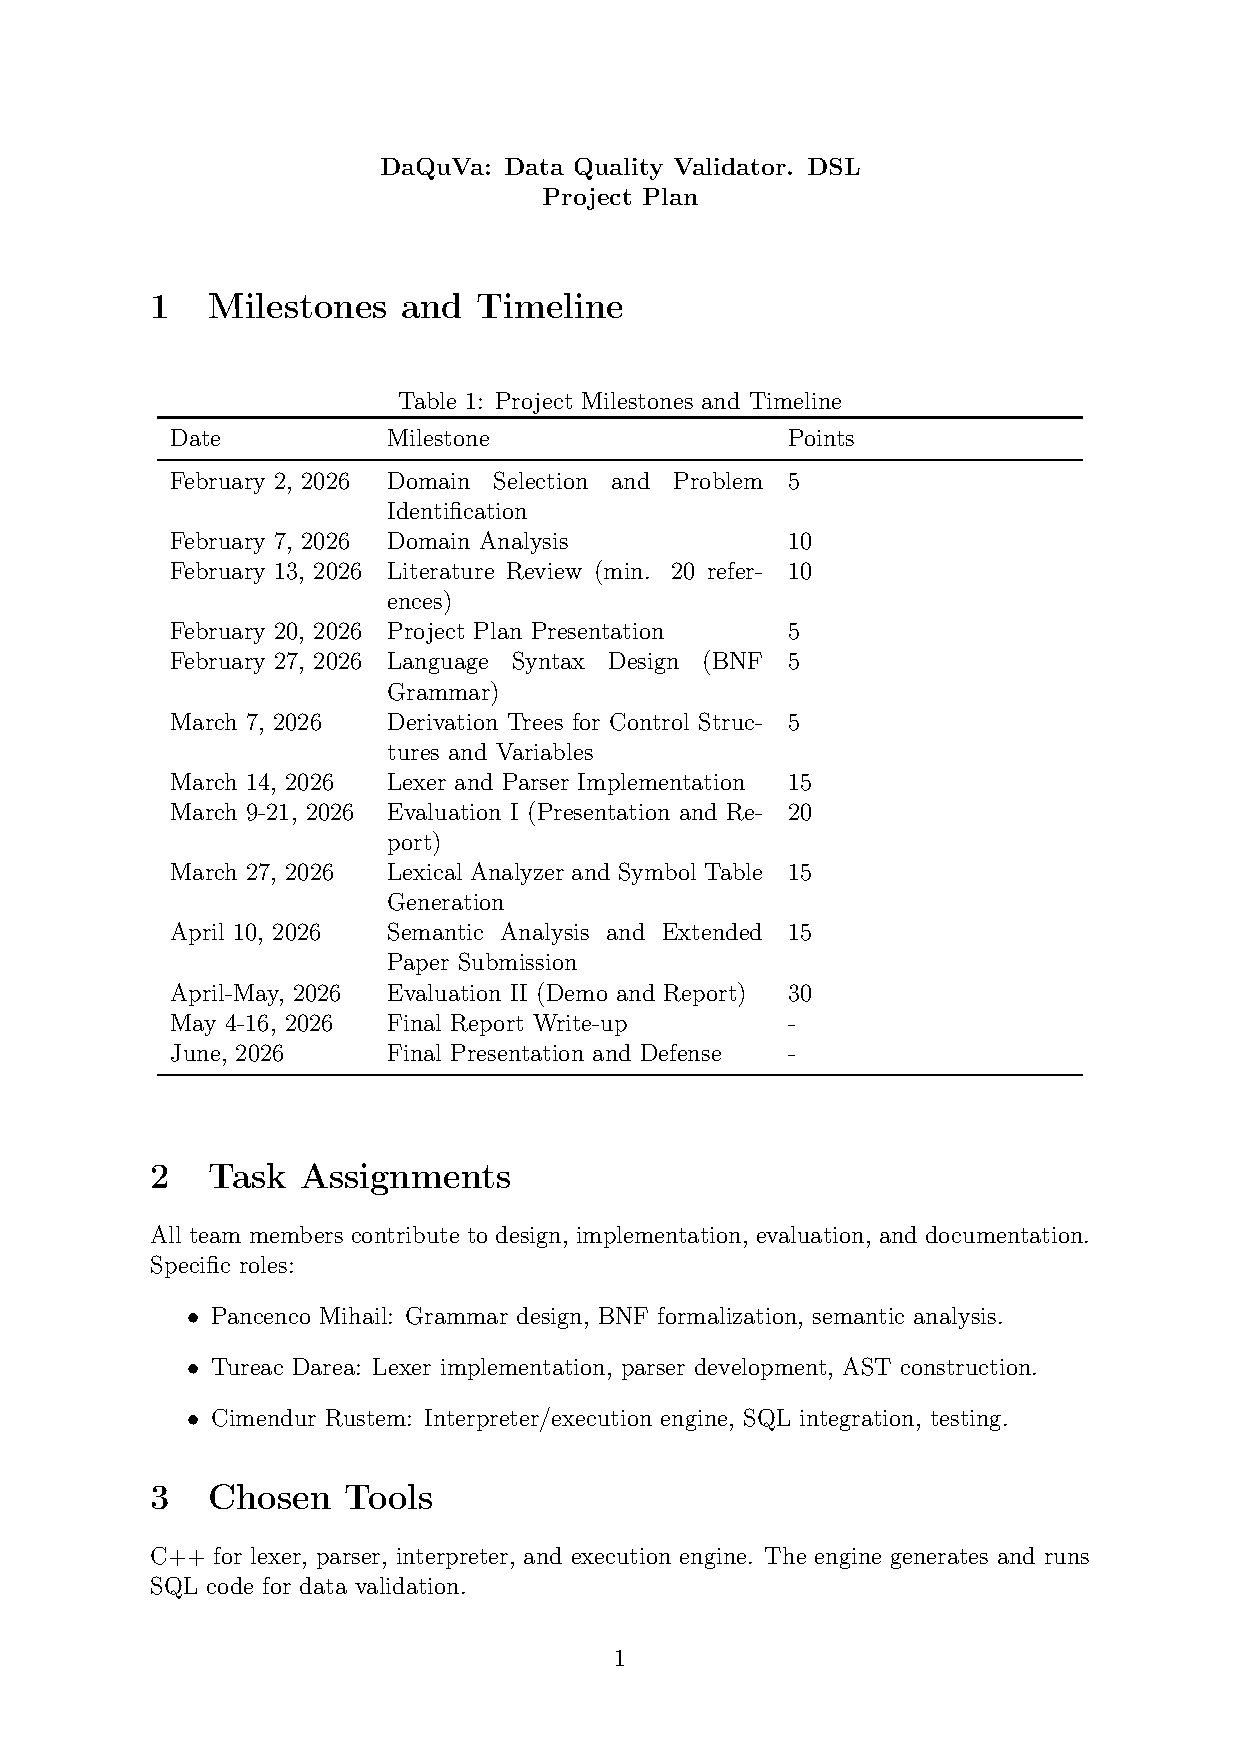
\includepdf[pages=1,
            width=\textwidth,
            height=0.82\textheight,
            keepaspectratio,
            pagecommand={\section{Project Plan}\thispagestyle{empty}}]{appendicies/project-plan.pdf}

% === Team Contract (1 page) ===
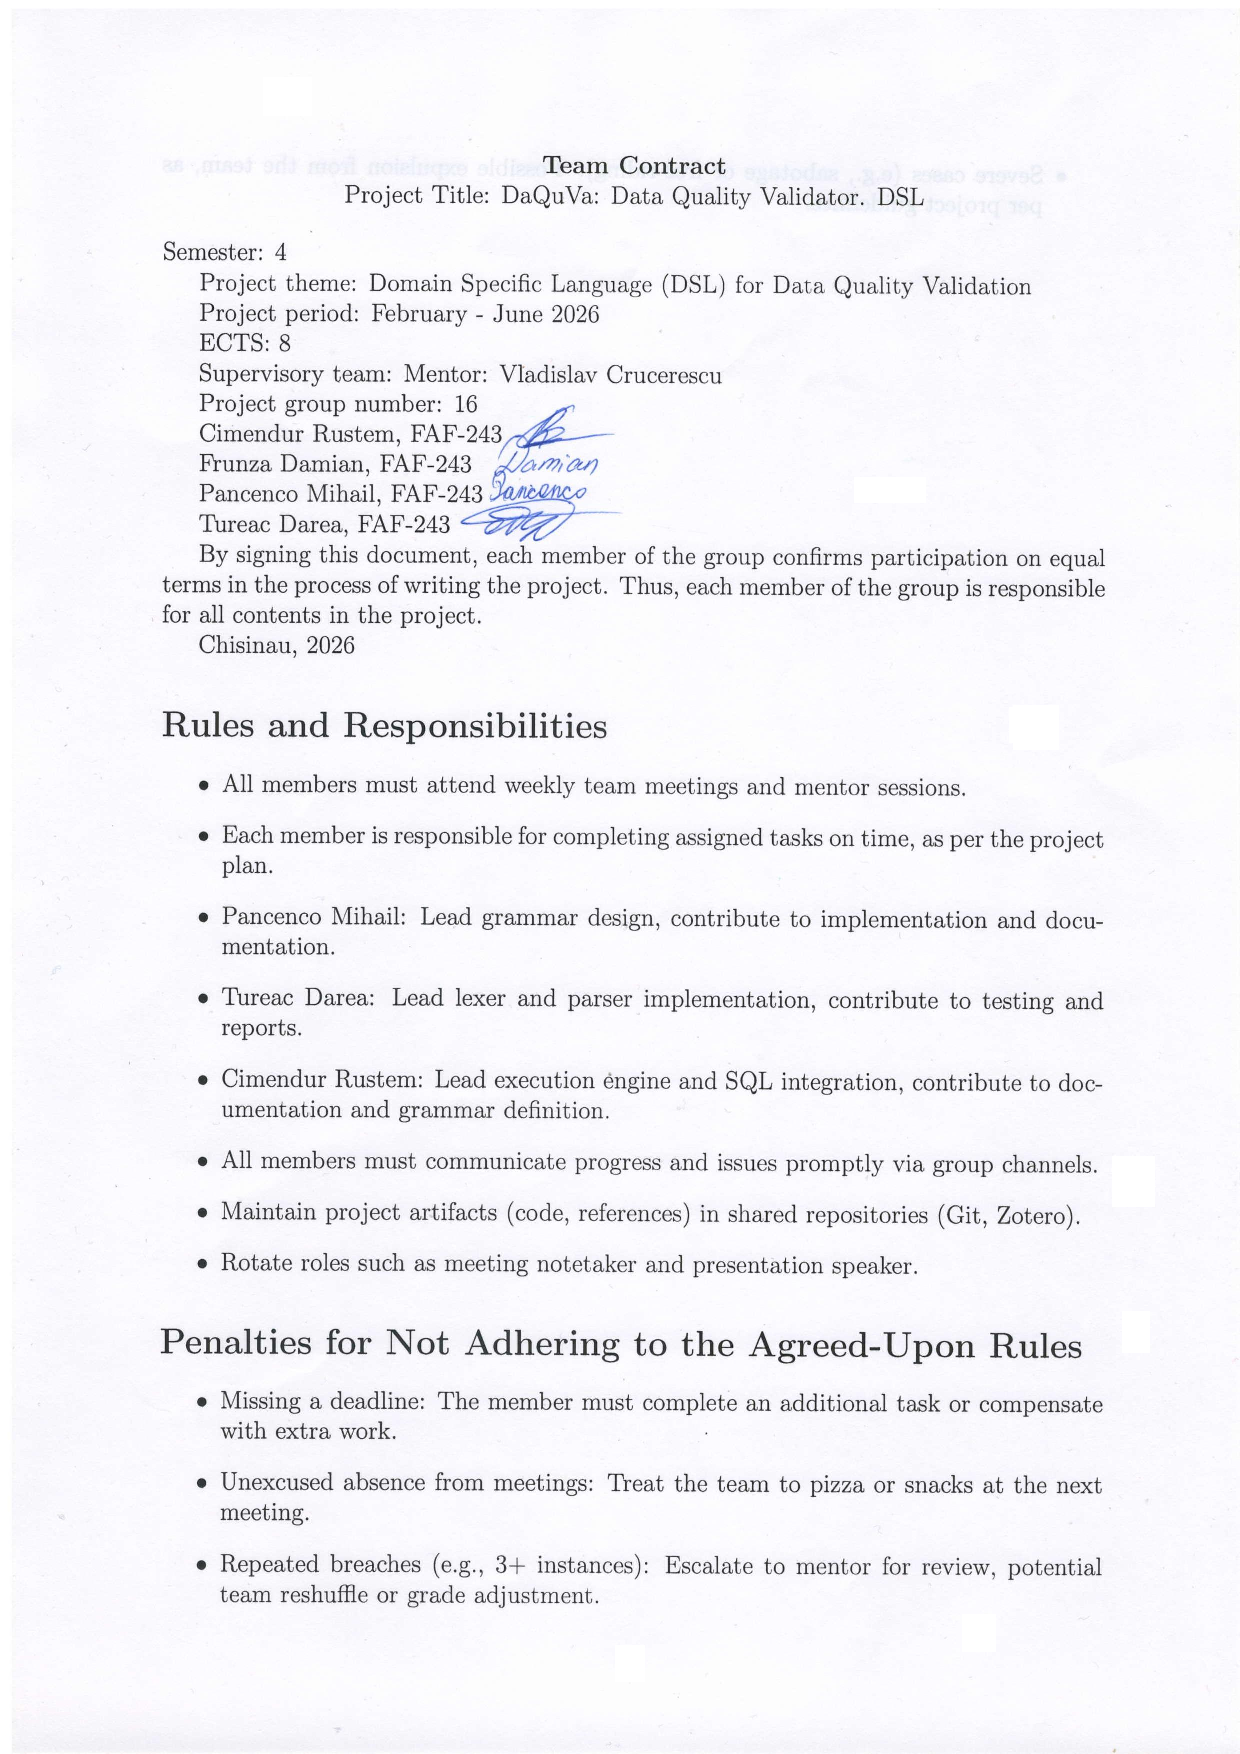
\includepdf[pages=1,
            width=\textwidth,
            height=0.82\textheight,
            keepaspectratio,
            pagecommand={\section{Team Contract}\thispagestyle{empty}}]{appendicies/team-contract.pdf}
    \clearpage
    
    \phantomsection
    \addcontentsline{toc}{chapter}{Bibliography}
    \nocite{*} 
    \bibliography{tex_files/bibliography/bibliography}

\end{document}